\documentclass[]{beamer}

% make header narrower
% \PassOptionsToPackage{height=2em}{beamerouterthemesidebar}

% needed for bold mathmode
\DeclareFontShape{OT1}{cmss}{b}{n}{<->ssub * cmss/bx/n}{}

\usepackage{changepage}
\usepackage{xspace}
\usepackage{soul}
\usepackage{amsfonts}
\usepackage{amsmath,amsfonts,amsthm} % Math packages
\usepackage{graphicx} % Allows including images
\usepackage{booktabs} % Allows the use of \toprule, \midrule and \bottomrule in tables
\usepackage{framed}
\usepackage{wrapfig}
\usepackage{caption}
\usepackage{tcolorbox}
\usepackage{arydshln}

\mode<presentation> {
\usepackage{subcaption}
\usepackage{algorithm,algorithmic}
\usepackage[titletoc,title]{appendix}
\usepackage{amsmath}
\usepackage{amsfonts}
\usepackage{amsmath,amssymb}
\usepackage{mathtools}
\captionsetup{compatibility=false}
\usepackage{blindtext}
\usepackage{tcolorbox}
\usepackage[final]{animate}
\usepackage{comment}
\usepackage{appendixnumberbeamer}
\usepackage{booktabs}
\usepackage{tikz}
\usetikzlibrary{calc,matrix}

\usetheme{AnnArbor}

\definecolor{myblue}{rgb}{0,0.156,0.375}
\definecolor{mymaize}{rgb}{1.,0.824,0.227}
\definecolor{beamer@myblue}{rgb}{0.02,0.1786,0.37109}
\definecolor{beamer@mymaize}{rgb}{1.,0.824,0.227}
\setbeamercolor{structure}{fg=beamer@myblue}
\setbeamercolor*{title}{use=structure,bg=beamer@mymaize,fg=beamer@myblue}
\setbeamercolor*{frametitle}{use=structure,bg=beamer@mymaize,fg=beamer@myblue}
\setbeamercolor*{palette primary}{use=structure,fg=beamer@mymaize,bg=beamer@myblue}
\setbeamercolor*{palette secondary}{use=structure,fg=beamer@mymaize,bg=beamer@myblue}
\setbeamercolor*{palette tertiary}{use=structure,fg=beamer@mymaize,bg=beamer@myblue}

\setbeamertemplate{frametitle}{%
    \nointerlineskip%
    \begin{beamercolorbox}[wd=\paperwidth,ht=2.5ex,dp=1ex]{frametitle}
        \hspace*{1ex}\insertframetitle%
    \end{beamercolorbox}%
}

\usepackage{appendixnumberbeamer}
\AtBeginSection[]{
  \begin{frame}
  \vfill
  \centering
  \begin{beamercolorbox}[sep=8pt,center,shadow=true,rounded=true]{title}
    \usebeamerfont{title}\insertsectionhead\par%
  \end{beamercolorbox}
  \vfill
  \end{frame}
}

\usepackage{textpos}
}

\newcommand*{\Scale}[2][4]{\scalebox{#1}{$#2$}}%
\newcommand*{\Resize}[2]{\resizebox{#1}{!}{$#2$}}%

% \addtobeamertemplate{frametitle}{}{%
% \begin{textblock*}{155mm}(-0.19\textwidth,-1.35cm)
% \end{textblock*}}

\usepackage{xcolor}

\beamertemplatenavigationsymbolsempty
\addtobeamertemplate{navigation symbols}{}{%
    \usebeamerfont{footline}%
    \usebeamercolor[fg]{footline}%
    \hspace{1em}%
    % \insertframenumber/\inserttotalframenumber
}

% Syntax: \colorboxed[<color model>]{<color specification>}{<math formula>}
\newcommand*{\colorboxed}{}
\def\colorboxed#1#{%
  \colorboxedAux{#1}%
}
\newcommand*{\colorboxedAux}[3]{%
  % #1: optional argument for color model
  % #2: color specification
  % #3: formula
  \begingroup
    \colorlet{cb@saved}{.}%
    \color#1{#2}%
    \boxed{%
      \color{cb@saved}%
      #3%
    }%
  \endgroup
}

\makeatletter
\newcommand{\miniscule}{\@setfontsize\miniscule{4}{5}}% \tiny: 5/6
\makeatother

\newcommand\blfootnote[1]{%
  \begingroup
  \renewcommand\thefootnote{}\footnote{#1}%
  \addtocounter{footnote}{-1}%
  \endgroup
}

\useoutertheme{miniframes}

\setbeamertemplate{navigation symbols}{}
\setbeamertemplate{section in head/foot shaded}{\color{gray}\usebeamertemplate{section in head/foot}}

\setbeamertemplate{headline}{%
  \begin{beamercolorbox}[colsep=1.5pt]{upper separation line head}
  \end{beamercolorbox}
  \begin{beamercolorbox}{section in head/foot}
    \vskip2pt\insertsectionnavigationhorizontal{\paperwidth}{}{}\vskip2pt
  \end{beamercolorbox}%
  \begin{beamercolorbox}[colsep=1.5pt]{lower separation line head}
  \end{beamercolorbox}
}

\newcommand{\MC}{\mathcal}
\renewcommand{\algorithmicrequire}{\textbf{Input:}}

% misc
\newcommand{\identMat}{\ensuremath{\mathbf{I}}}
\newcommand{\zeroVec}{\ensuremath{\mathbf{0}}}
\newcommand{\volume}{\ooalign{\hfil$V$\hfil\cr\kern0.08em--\hfil\cr}}
\newcommand{\norm}[1]{\ensuremath{\left\lVert#1\right\rVert}}
\newcommand{\defEq}{\ensuremath{:=}}
\newcommand{\standardstate}{\circ\kern-0.47em-}
\newcommand{\CC}{C\nolinebreak[4]\hspace{-.05em}\raisebox{.4ex}{\relsize{-3}{\textbf{++}}}}
\newcommand{\canonVec}{\ensuremath{\mathbf{e}}}

% time
\newcommand{\timeVar}{\ensuremath{\text{t}}}
\newcommand{\initTime}{\ensuremath{\timeVar^0}}
\newcommand{\dt}{\ensuremath{\Delta \timeVar}}
\newcommand{\dtFOM}{\ensuremath{\Delta \timeVar_{\text{FOM}}}}
\newcommand{\dtau}{\ensuremath{\Delta \tau}}
\newcommand{\finalTime}{\ensuremath{\text{T}}}
\newcommand{\dott}[1]{\accentset{\mbox{\large\bfseries .}}{#1}}

% indices
\newcommand{\spatialIdx}{\ensuremath{i}}
\newcommand{\spatialIdxTwo}{\ensuremath{j}}
\newcommand{\spatialIdxThree}{\ensuremath{k}}
\newcommand{\spatialIdxFour}{\ensuremath{m}}
\newcommand{\specIdx}{\ensuremath{l}}
\newcommand{\specIdxTwo}{\ensuremath{m}}
\newcommand{\timeIdx}{\ensuremath{n}}
\newcommand{\newtonIdx}{\ensuremath{k}}
\newcommand{\reacIdx}{\ensuremath{r}}
\newcommand{\varIdx}{\ensuremath{v}}
\newcommand{\greedyIdx}{\ensuremath{m}}
\newcommand{\sampIdx}{\ensuremath{s}}

% dimensions
\newcommand{\numDOF}{\ensuremath{N}}
\newcommand{\numSpec}{\ensuremath{N_Y}}
\newcommand{\numConsModes}{\ensuremath{N_c}}
\newcommand{\numPrimModes}{\ensuremath{N_p}}
\newcommand{\numRHSModes}{\ensuremath{N_f}}
\newcommand{\numResModes}{\ensuremath{N_r}}
\newcommand{\numJacobModes}{\ensuremath{N_J}}
\newcommand{\numSamps}{\ensuremath{N_s}}
\newcommand{\numSampsFull}{\ensuremath{\widetilde{N}_s}}
\newcommand{\numReacs}{\ensuremath{N_r}}
\newcommand{\numSnaps}{\ensuremath{N_{\finalTime}}}
\newcommand{\numProg}{\ensuremath{N_{\text{prog}}}}
\newcommand{\numLayers}{\ensuremath{N_{L}}}
\newcommand{\numNNInput}{\ensuremath{N_{I}}}
\newcommand{\numNNOutput}{\ensuremath{N_{O}}}
\newcommand{\numVars}{\ensuremath{N_{v}}}
\newcommand{\numCells}{\ensuremath{N_{e}}}

% spatial coordinates
\newcommand{\spatialVar}{\ensuremath{x}}
\newcommand{\spatialVec}{\ensuremath{\mathbf{x}}}
\newcommand{\spatialVarDir}{\ensuremath{\spatialVar_{\spatialIdx}}}

% state variables
\newcommand{\stateVar}{q}
\newcommand{\stateVec}{\ensuremath{\mathbf{\stateVar}}}
\newcommand{\stateVecVar}{\ensuremath{\mathbf{\stateVar}_{\varIdx}}}
\newcommand{\consVar}{c}
\newcommand{\primVar}{p}
\newcommand{\consVec}{\ensuremath{\mathbf{\stateVar}_{\consVar}}}
\newcommand{\consVecVar}{\ensuremath{\mathbf{\stateVar}_{\consVar,\varIdx}}}
\newcommand{\primVec}{\ensuremath{\mathbf{\stateVar}_{\primVar}}}
\newcommand{\primVecVar}{\ensuremath{\mathbf{\stateVar}_{\primVar,\varIdx}}}
\newcommand{\consFunc}[1]{\ensuremath{\consVec \left(#1\right)}}
\newcommand{\consFuncUns}[1]{\ensuremath{\consVec' \left(#1\right)}}
\newcommand{\primFuncUns}[1]{\ensuremath{\primVec' \left(#1\right)}}
\newcommand{\stateVecCent}{\ensuremath{\mathbf{\overline{\stateVar}}}}
\newcommand{\consValCentVar}{\ensuremath{\overline{\stateVar}_{\consVar,\varIdx}}}
\newcommand{\consVecCent}{\ensuremath{\mathbf{\overline{\stateVar}}_{\consVar}}}
\newcommand{\consVecCentVar}{\ensuremath{\mathbf{\overline{\stateVar}}_{\consVar,\varIdx}}}
\newcommand{\primFunc}[1]{\ensuremath{\primVec \left(#1\right)}}
\newcommand{\primVecCent}{\ensuremath{\mathbf{\overline{\stateVar}}_{\primVar}}}
\newcommand{\primVecCentVar}{\ensuremath{\mathbf{\overline{\stateVar}}_{\primVar,\varIdx}}}
\newcommand{\primValCentVar}{\ensuremath{\overline{\stateVar}_{\primVar,\varIdx}}}
\newcommand{\consDataMat}{\ensuremath{\mathbf{\MakeUppercase{\stateVar}}_{\consVar}}}
\newcommand{\consDataMatUns}{\ensuremath{\consDataMat'}}
\newcommand{\consDataMatVar}{\ensuremath{\mathbf{\MakeUppercase{\stateVar}}_{\consVar,\varIdx}}}
\newcommand{\primDataMat}{\ensuremath{\mathbf{\MakeUppercase{\stateVar}}_{\primVar}}}
\newcommand{\primDataMatUns}{\ensuremath{\primDataMat'}}
\newcommand{\primDataMatVar}{\ensuremath{\mathbf{\MakeUppercase{\stateVar}}_{\primVar,\varIdx}}}
\newcommand{\rkVec}{\ensuremath{\mathbf{h}}}
\newcommand{\consVecDt}{\ensuremath{\dott{\mathbf{\stateVar}}_{\consVar}}}
\newcommand{\consVecRomDt}{\ensuremath{\dott{\mathbf{\widetilde{\stateVar}}}_{\consVar}}}
\newcommand{\consVecCoefDt}{\ensuremath{\dott{\mathbf{\widehat{\stateVar}}}_{\consVar}}}
\newcommand{\solutionVar}{t}
\newcommand{\targetVec}{\ensuremath{\mathbf{\stateVar}_{\targetVar}}}

% dummies
\newcommand{\dummyVecVar}{y}
\newcommand{\dummyVec}{\ensuremath{\mathbf{\dummyVecVar}}}
\newcommand{\dummyVecOne}{\ensuremath{\mathbf{a}}}
\newcommand{\dummyVecTwo}{\ensuremath{\mathbf{b}}}
\newcommand{\dummyIdx}{\ensuremath{i}}
\newcommand{\dummyIdxTwo}{\ensuremath{j}}
\newcommand{\dummyMat}{\ensuremath{\mathbf{A}}}
\newcommand{\dummyMatOne}{\ensuremath{\mathbf{A}}}
\newcommand{\dummyMatTwo}{\ensuremath{\mathbf{B}}}
\newcommand{\dummyMatThree}{\ensuremath{\mathbf{C}}}
\newcommand{\dummyMatFour}{\ensuremath{\mathbf{D}}}
\newcommand{\dummyMatFive}{\ensuremath{\mathbf{E}}}
\newcommand{\dummyMatSix}{\ensuremath{\mathbf{G}}}
\newcommand{\dummyMatSeven}{\ensuremath{\mathbf{H}}}
\newcommand{\dummyMatEight}{\ensuremath{\mathbf{K}}}

% ROM variables
\newcommand{\consVecRom}{\ensuremath{\mathbf{\widetilde{\stateVar}}_{\consVar}}}
\newcommand{\consVecRomVar}{\ensuremath{\mathbf{\widetilde{\stateVar}}_{{\consVar},\varIdx}}}
\newcommand{\consFuncRom}[1]{\ensuremath{\consVecRom \left(#1\right)}}
\newcommand{\primVecRom}{\ensuremath{\mathbf{\widetilde{\stateVar}}_{\primVar}}}
\newcommand{\primFuncRom}[1]{\ensuremath{\primVecRom \left(#1\right)}}
\newcommand{\primVecRomVar}{\ensuremath{\mathbf{\widetilde{\stateVar}}_{\primVar,\varIdx}}}
\newcommand{\stateVecCoef}{\ensuremath{\mathbf{\widehat{\stateVar}}}}
\newcommand{\consVecCoef}{\ensuremath{\mathbf{\widehat{\stateVar}}_{\consVar}}}
\newcommand{\consVarCoef}[1]{\ensuremath{\widehat{\stateVar}_{\consVar,#1}}}
\newcommand{\consVarCoefIdx}{\ensuremath{\widehat{\stateVar}_{\consVar,\dummyIdx}}}
\newcommand{\primVecCoef}{\ensuremath{\mathbf{\widehat{\stateVar}}_{\primVar}}}
\newcommand{\primVarCoef}[1]{\ensuremath{\widehat{\stateVar}_{\primVar,#1}}}
\newcommand{\primVarCoefIdx}{\ensuremath{\widehat{\stateVar}}_{\primVar,\dummyIdx}}

% flux/source/RHS/residual functions
\newcommand{\fluxVar}{\ensuremath{f}}
\newcommand{\invFlux}{\ensuremath{\mathbf{\fluxVar}}}
\newcommand{\viscFlux}{\ensuremath{\mathbf{\fluxVar}_{\nu}}}
\newcommand{\invFluxDir}{\ensuremath{\mathbf{\fluxVar}_{\spatialIdx}}}
\newcommand{\viscFluxDir}{\ensuremath{\mathbf{\fluxVar}_{\nu,\spatialIdx}}}
\newcommand{\viscFluxDirArg}[1]{\ensuremath{\mathbf{\fluxVar}_{\nu,#1}}}
\newcommand{\sourceVar}{\ensuremath{s}}
\newcommand{\sourceVec}{\mathbf{\sourceVar}}
\newcommand{\rhsVar}{f}
\newcommand{\rhsVec}{\ensuremath{\mathbf{\rhsVar}}}
\newcommand{\rhsFunc}[1]{\ensuremath{\rhsVec \left(#1\right)}}
\newcommand{\rhsApproxVec}{\ensuremath{\mathbf{\widetilde{\rhsVar}}}}
\newcommand{\rhsApproxFunc}[1]{\ensuremath{\mathbf{\widetilde{\rhsVar}}\left(#1\right)}}
\newcommand{\resVar}{r}
\newcommand{\resVec}{\ensuremath{\mathbf{\resVar}}}
\newcommand{\resFunc}[1]{\ensuremath{\resVec\left(#1\right)}}
\newcommand{\resFuncIter}[2]{\ensuremath{\resVec^{#1}\left(#2\right)}}
\newcommand{\resApproxVec}{\ensuremath{\mathbf{\widetilde{\resVar}}}}
\newcommand{\resApproxFunc}[1]{\ensuremath{\mathbf{\widetilde{\resVar}}\left(#1\right)}}
\newcommand{\resApproxFuncIter}[2]{\ensuremath{\mathbf{\widetilde{\resVar}}^{#1} \left(#2\right)}}
\newcommand{\sampFunc}[1]{\ensuremath{\mathbf{s}\left(#1\right)}}
\newcommand{\rhsResVec}{\ensuremath{\mathbf{\rhsVar}_{\resVec}}}
\newcommand{\rhsResFunc}[1]{\ensuremath{\mathbf{\rhsVar}_{\resVec}\left(#1\right)}}
\newcommand{\rhsResApproxFunc}[1]{\ensuremath{\mathbf{\widetilde{\rhsVar}}_{\resVec}\left(#1\right)}}
\newcommand{\rhsDataMat}{\ensuremath{\mathbf{\MakeUppercase{\rhsVar}}}}
\newcommand{\resDataMat}{\ensuremath{\mathbf{\MakeUppercase{\resVar}}}}

% non-linear functions
\newcommand{\encoderVar}{\ensuremath{h}}
\newcommand{\encoder}{\ensuremath{\mathbf{\encoderVar}}}
\newcommand{\encoderFunc}[1]{\ensuremath{\encoder \left(#1\right)}}
\newcommand{\decoderVar}{\ensuremath{g}}
\newcommand{\decoder}{\ensuremath{\mathbf{\decoderVar}}}
\newcommand{\decoderFunc}[1]{\ensuremath{\decoder \left(#1\right)}}
\newcommand{\nnInput}{\ensuremath{\mathbf{x}}}
\newcommand{\nnInputApprox}{\ensuremath{\mathbf{\widetilde{x}}}}
\newcommand{\nnInputCoef}{\ensuremath{\mathbf{\widehat{x}}}}
\newcommand{\nnOutput}{\ensuremath{\mathbf{y}}}
% \newcommand{\nnLayerVar}{g}
% \newcommand{\nnLayer}{\ensuremath{\mathbf{\nnLayerVar}}}
\newcommand{\nnLayerVar}{\ensuremath{\varphi}}
\newcommand{\nnLayer}{\ensuremath{\boldsymbol{\nnLayerVar}}}
\newcommand{\trialConsMap}{\nnLayer_{\decoderVar, \consVar}}
\newcommand{\trialConsFunc}[1]{\trialConsMap\left(#1\right)}
\newcommand{\trialPrimMap}{\nnLayer_{\decoderVar, \primVar}}
\newcommand{\trialPrimFunc}[1]{\trialPrimMap \left(#1\right)}
\newcommand{\nnLayerIdx}[1]{\ensuremath{\nnLayer^{#1}}}
\newcommand{\nnLayerFunc}[1]{\ensuremath{\nnLayer\left({#1}\right)}}
\newcommand{\nnLayerFuncIdx}[2]{\ensuremath{\nnLayer^{#2}\left({#1}\right)}}
\newcommand{\nnAct}{\ensuremath{\boldsymbol{\sigma}}}
\newcommand{\actFunc}[1]{\ensuremath{\nnAct\left(#1\right)}}
\newcommand{\nnParams}{\ensuremath{\boldsymbol{\Theta}}}
\newcommand{\nnWeights}{\ensuremath{\mathbf{W}}}
\newcommand{\nnBias}{\ensuremath{\mathbf{b}}}
\newcommand{\nnCost}{\ensuremath{c}}
\newcommand{\nnCostFunc}[1]{\ensuremath{\nnCost\left(#1\right)}}


% Jacobians
\newcommand{\jacobMat}{\ensuremath{\mathbf{J}}}
\newcommand{\jacobTrialCons}{\ensuremath{\jacobMat_{\nnLayerVar,\consVar}}}
\newcommand{\jacobTrialPrim}{\ensuremath{\jacobMat_{\nnLayerVar,\primVar}}}
\newcommand{\jacobDecodeCons}{\ensuremath{\consScale \jacobTrialCons}}
\newcommand{\jacobDecodePrim}{\ensuremath{\primScale \jacobTrialPrim}}
\newcommand{\jacobMatCoef}{\ensuremath{\mathbf{\widehat{J}}}}
\newcommand{\jacobResCons}{\ensuremath{\jacobMat_{\resVar,\consVar}}}
\newcommand{\jacobResPrim}{\ensuremath{\jacobMat_{\resVar,\primVar}}}
\newcommand{\jacobResCoefCons}{\ensuremath{\jacobMatCoef_{\resVar,\consVar}}}
\newcommand{\jacobResCoefPrim}{\ensuremath{\jacobMatCoef_{\resVar,\primVar}}}
\newcommand{\jacobCons}{\ensuremath{\jacobMat_{\consVar}}}
\newcommand{\jacobPrim}{\ensuremath{\jacobMat_{\primVar}}}
\newcommand{\jacobTrialConsFunc}[1]{\ensuremath{\jacobTrialCons \left(#1\right)}}
\newcommand{\jacobTrialPrimFunc}[1]{\ensuremath{\jacobTrialPrim \left(#1\right)}}
\newcommand{\jacobDecodeConsFunc}[1]{\ensuremath{\jacobDecodeCons \left(#1\right)}}
\newcommand{\jacobDecodePrimFunc}[1]{\ensuremath{\jacobDecodePrim \left(#1\right)}}
\newcommand{\jacobApproxFunc}[1]{\ensuremath{\widetilde{\jacobMat}}\left(#1\right)}
\newcommand{\gm}{\ensuremath{\boldsymbol{\Gamma}}}
\newcommand{\gmFunc}[1]{\ensuremath{\gm \left(#1\right)}}
\newcommand{\gmInv}{\ensuremath{\boldsymbol{\Gamma}^{-1}}}

% linear bases
\newcommand{\basisVar}{u}
\newcommand{\basisMat}{\ensuremath{\mathbf{\MakeUppercase{\basisVar}}}}
\newcommand{\consTrial}{\ensuremath{\basisMat}_{\consVar}}
\newcommand{\consTrialVecIdx}{\ensuremath{\mathbf{\basisVar}}_{\consVar,\dummyIdx}}
\newcommand{\consTrialVec}[1]{\ensuremath{\mathbf{\basisVar}}_{\consVar,#1}}
\newcommand{\consTrialUpdate}{\ensuremath{\basisMat}'_{\consVar}}
\newcommand{\primTrial}{\ensuremath{\basisMat_p}}
\newcommand{\primTrialVecIdx}{\ensuremath{\mathbf{\basisVar}}_{\primVar,\dummyIdx}}
\newcommand{\primTrialVec}[1]{\ensuremath{\mathbf{\basisVar}}_{\primVar,#1}}
\newcommand{\rightSingVecVar}{v}
\newcommand{\rightSingVecMat}{\ensuremath{\mathbf{\MakeUppercase{\rightSingVecVar}}}}
\newcommand{\singVecMat}{\ensuremath{\boldsymbol{\Sigma}}}
\newcommand{\testBasisVar}{w}
\newcommand{\testBasisMat}{\ensuremath{\mathbf{\MakeUppercase{\testBasisVar}}}}
\newcommand{\testBasis}{\ensuremath{\testBasisMat}}
\newcommand{\testBasisCons}{\ensuremath{\mathbf{\MakeUppercase{\testBasisVar}}_{\consVar}}}
\newcommand{\testBasisPrim}{\ensuremath{\mathbf{\MakeUppercase{\testBasisVar}}_{\primVar}}}
\newcommand{\testBasisFunc}[1]{\ensuremath{\testBasisMat}\left(#1\right)}
\newcommand{\testBasisApproxFunc}[1]{\ensuremath{\widetilde{\testBasisMat}}\left(#1\right)}

% DEIM
\newcommand{\deimBasisVar}{\ensuremath{\Psi}}
\newcommand{\deimBasisVec}{\ensuremath{\boldsymbol{\psi}}}
\newcommand{\deimBasisMat}{\ensuremath{\mathbf{\MakeUppercase{\deimBasisVar}}}}
\newcommand{\deimBasisCons}{\ensuremath{\deimBasisMat_{\consVar}}}
\newcommand{\deimBasisRhs}{\ensuremath{\deimBasisMat_{\rhsVar}}}
\newcommand{\deimBasis}{\ensuremath{\deimBasisMat}}
\newcommand{\deimBasisRes}{\ensuremath{\deimBasisMat_{\resVec}}}
\newcommand{\deimBasisJacob}{\ensuremath{\deimBasisMat_{\jacobMat}}}
\newcommand{\sampVec}{\ensuremath{\mathbf{s}}}
\newcommand{\sampMat}{\ensuremath{\mathbf{S}}}
\newcommand{\sampMatFull}{\ensuremath{\mathbf{\widetilde{S}}}}
\newcommand{\sampMatComp}{\ensuremath{\mathbf{\breve{S}}}}
\newcommand{\sampMatInterp}{\ensuremath{\mathbf{\widehat{S}}}}
\newcommand{\sampSet}{\ensuremath{\MC{S}}}
\newcommand{\sampSetFull}{\ensuremath{\MC{\widetilde{S}}}}
\newcommand{\deimRegressorCons}{\ensuremath{\deimBasisCons (\sampMat \deimBasisCons)^+ \sampMat}}
\newcommand{\deimRegressorConsSmall}{\ensuremath{(\sampMat \deimBasisCons)^+ \sampMat}}
\newcommand{\deimRegressorConsTiny}{\ensuremath{(\sampMat \deimBasisCons)^+}}
\newcommand{\deimRegressorRhs}{\ensuremath{\deimBasisRhs (\sampMat \deimBasisRhs)^+ \sampMat}}
\newcommand{\deimRegressorRhsSmall}{\ensuremath{(\sampMat \deimBasisRhs)^+ \sampMat}}
\newcommand{\deimRegressorRhsTiny}{\ensuremath{(\sampMat \deimBasisRhs)^+}}
\newcommand{\deimRegressorRes}{\ensuremath{\deimBasisRes (\sampMat \deimBasisRes)^+ \sampMat}}
\newcommand{\deimRegressorResSmall}{\ensuremath{(\sampMat \deimBasisRes)^+ \sampMat}}
\newcommand{\deimRegressorJac}{\ensuremath{\deimBasisJac (\sampMat \deimBasisJac)^+ \sampMat}}
\newcommand{\deimRegressorJacSmall}{\ensuremath{(\sampMat \deimBasisJac)^+ \sampMat}}
\newcommand{\deimBasisREvecRow}{\ensuremath{\deimBasisVec'_+}}
\newcommand{\deimBasisRowUpdate}{\ensuremath{\deimBasisVec_+}}

% AADEIM
\newcommand{\adeimAlpha}{\ensuremath{\boldsymbol{\alpha}}}
\newcommand{\adeimBeta}{\ensuremath{\boldsymbol{\beta}}}
\newcommand{\resWindow}{\ensuremath{\mathbf{\MakeUppercase{\rhsVar}}_{\resVar}}}
\newcommand{\numWindow}{w}
\newcommand{\numRank}{z}

% SVD
\newcommand{\lEvecVar}{x}
\newcommand{\rEvecVar}{y}
\newcommand{\singVal}{\ensuremath{\sigma}}
\newcommand{\leftEvecMat}{\ensuremath{\ensuremath{\mathbf{\MakeUppercase{\lEvecVar}}}}}
\newcommand{\singValMat}{\ensuremath{\boldsymbol{\Sigma}}}
\newcommand{\rightEvecMat}{\ensuremath{\ensuremath{\mathbf{\MakeUppercase{\rEvecVar}}}}}
\newcommand{\eigenVal}{\ensuremath{\lambda}}

% spaces/manifolds
\newcommand{\trialSpace}{\ensuremath{\widetilde{\MC{\MakeUppercase{\basisVar}}}}}
\newcommand{\consTrialSpace}{\ensuremath{\trialSpace_{\consVar}}}
\newcommand{\primTrialSpace}{\ensuremath{\trialSpace_{\primVar}}}

% scaling matrices
% \newcommand{\consScaleVar}{p}
% \newcommand{\consScale}{\ensuremath{\mathbf{\MakeUppercase{\consScaleVar}}}}
% \newcommand{\consScaleInv}{\ensuremath{\consScale^{-1}}}
% \newcommand{\primScaleVar}{h}
% \newcommand{\primScale}{\ensuremath{\mathbf{\MakeUppercase{\primScaleVar}}}}
% \newcommand{\primScaleInv}{\ensuremath{\primScale^{-1}}}
\newcommand{\scaleVar}{h}
\newcommand{\scaleMat}{\ensuremath{\mathbf{\MakeUppercase{\scaleVar}}}}
\newcommand{\scaleVec}{\ensuremath{\mathbf{\scaleVar}}}
\newcommand{\scaleMatInv}{\ensuremath{\scaleMat^{-1}}}
\newcommand{\consScaleVar}[1]{\ensuremath{\scaleVar_{\consVar,#1}}}
\newcommand{\consScaleVecVar}[1]{\ensuremath{\scaleVec_{\consVar,#1}}}
\newcommand{\consScale}{\ensuremath{\scaleMat_{\consVar}}}
\newcommand{\consScaleInv}{\ensuremath{\consScale^{-1}}}
\newcommand{\primScaleVar}[1]{\ensuremath{\scaleVar_{\primVar,#1}}}
\newcommand{\primScaleVecVar}[1]{\ensuremath{\scaleVec_{\primVar,#1}}}
\newcommand{\primScale}{\ensuremath{\scaleMat_{\primVar}}}
\newcommand{\primScaleInv}{\ensuremath{\primScale^{-1}}}
\newcommand{\rhsScaleVar}{g}
\newcommand{\rhsScale}{\ensuremath{\mathbf{\MakeUppercase{\rhsScaleVar}}}}
\newcommand{\rhsScaleInv}{\ensuremath{\rhsScale^{-1}}}
\newcommand{\resScaleVar}{r}
\newcommand{\resScale}{\ensuremath{\mathbf{\MakeUppercase{\resScaleVar}}}}
\newcommand{\resScaleInv}{\ensuremath{\resScale^{-1}}}

% error
\newcommand{\errVec}{\ensuremath{\epsilon}}
\newcommand{\errVecVar}{\ensuremath{\errVec_{\varIdx}}}

% thermodynamic quantities
\newcommand{\density}{\ensuremath{\rho}}
\newcommand{\enth}{\ensuremath{h}}
\newcommand{\stagEnth}{\ensuremath{\enth^0}}
\newcommand{\enthSpec}{\ensuremath{\enth_{\specIdx}}}
\newcommand{\refEnth}{\ensuremath{\enth^{\standardstate}}}
\newcommand{\refEnthSpec}{\ensuremath{\enth^{\standardstate}_{\specIdx}}}
\newcommand{\entropy}{\ensuremath{s}}
\newcommand{\entropySpec}{\ensuremath{\entropy_{\specIdx}}}
\newcommand{\shearStress}{\ensuremath{\tau}}
\newcommand{\cp}{\ensuremath{c_{p}}}
\newcommand{\cpSpec}{\ensuremath{c_{p,\specIdx}}}
\newcommand{\gibbs}{\ensuremath{g}}
\newcommand{\gibbsSpec}{\ensuremath{g}_{\specIdx}}
\newcommand{\pressure}{\ensuremath{p}}
\newcommand{\pressureBack}{\ensuremath{p_b}}
\newcommand{\pressureMean}{\ensuremath{\overline{p}}}
\newcommand{\temperature}{\ensuremath{T}}
\newcommand{\tempReduced}{\ensuremath{T^*}}
\newcommand{\heatFlux}{\ensuremath{q}}
\newcommand{\vel}{\ensuremath{u}}
\newcommand{\velX}{\ensuremath{u}}
\newcommand{\velY}{\ensuremath{v}}
\newcommand{\velZ}{\ensuremath{w}}
\newcommand{\fitScalOneVar}{\ensuremath{a}}
\newcommand{\fitScalOneSpec}[1]{\ensuremath{\fitScalOneVar_{#1,\specIdx}}}
\newcommand{\fitScalTwoVar}{\ensuremath{b}}
\newcommand{\fitScalTwoSpec}[1]{\ensuremath{\fitScalTwoVar_{#1,\specIdx}}}
\newcommand{\fitScalThreeVar}{\ensuremath{c}}
\newcommand{\fitScalThreeSpec}[1]{\ensuremath{\fitScalThreeVar_{#1,\specIdx}}}
\newcommand{\fitScalFourVar}{\ensuremath{d}}
\newcommand{\fitScalFour}[1]{\ensuremath{\fitScalFourVar_{#1}}}
\newcommand{\fitScalFourSpec}[1]{\ensuremath{\fitScalFourVar_{#1,\specIdx}}}
\newcommand{\fitScalFourSpecTwo}[1]{\ensuremath{\fitScalFourVar_{#1,\specIdx \specIdxTwo}}}

% chemical quantities
\newcommand{\mf}{\ensuremath{Y}}
\newcommand{\mfSpec}{\ensuremath{\mf_{\specIdx}}}
\newcommand{\mfSpecTwo}{\ensuremath{\mf_{\specIdxTwo}}}
\newcommand{\mole}{\ensuremath{X}}
\newcommand{\moleSpec}{\ensuremath{\mole_{\specIdx}}}
\newcommand{\moleSpecTwo}{\ensuremath{\mole_{\specIdxTwo}}}
\newcommand{\moleConcSpec}{\ensuremath{[\moleSpec]}}
\newcommand{\mw}{\ensuremath{M}}
\newcommand{\mwSpec}{\ensuremath{\mw_{\specIdx}}}
\newcommand{\mwSpecTwo}{\ensuremath{\mw_{\specIdxTwo}}}
\newcommand{\gasConst}{\ensuremath{R}}
\newcommand{\gasConstSpec}{\ensuremath{\gasConst_{\specIdx}}}
\newcommand{\gasConstUniv}{\ensuremath{\gasConst_u}}
\newcommand{\mixFrac}{Z}
\newcommand{\progVar}{C}

% transport quantities
\newcommand{\diffVelVar}{\ensuremath{V}}
\newcommand{\diffVelDir}{\ensuremath{\diffVelVar_{\spatialIdx, \specIdx}}}
\newcommand{\massDiffVar}{\ensuremath{D}}
\newcommand{\massDiffSpec}{\ensuremath{\massDiffVar_{\specIdx M}}}
\newcommand{\massDiffSpecTwo}{\ensuremath{\massDiffVar_{\specIdx, \specIdxTwo}}}
\newcommand{\massDiffMixFrac}{\ensuremath{\massDiffVar_{\mixFrac}}}
\newcommand{\massDiffProgVar}{\ensuremath{\massDiffVar_{\progVar}}}
\newcommand{\dynVisc}{\ensuremath{\mu}}
\newcommand{\dynViscSpec}{\ensuremath{\dynVisc_{\specIdx}}}
\newcommand{\dynViscSpecTwo}{\ensuremath{\dynVisc_{\specIdxTwo}}}
\newcommand{\dynViscRefSpec}{\ensuremath{\dynVisc_{\text{ref},\specIdx}}}
\newcommand{\tempRefSpec}{\ensuremath{T_{\text{ref},\specIdx}}}
\newcommand{\suthTemp}{\ensuremath{S}}
\newcommand{\suthTempSpec}{\suthTemp_{\specIdx}}
\newcommand{\constVisc}{\ensuremath{\overline{\dynVisc}}}
\newcommand{\constViscSpec}{\ensuremath{\constVisc_{\specIdx}}}
\newcommand{\thermCond}{\ensuremath{\lambda}}
\newcommand{\thermCondSpec}{\ensuremath{\thermCond_{\specIdx}}}
\newcommand{\ljEnergy}{\ensuremath{\epsilon}}
\newcommand{\ljEnergySpec}{\ensuremath{\ljEnergy_{\specIdx}}}
\newcommand{\ljEnergySpecTwo}{\ensuremath{\ljEnergy_{\specIdxTwo}}}
\newcommand{\ljPotential}{\ensuremath{\Omega}}
\newcommand{\collisionDiam}{\ensuremath{\sigma}}
\newcommand{\collisionDiamSpec}{\ensuremath{\sigma_{\specIdx}}}
\newcommand{\collisionDiamSpecTwo}{\ensuremath{\sigma_{\specIdxTwo}}}
\newcommand{\diffusionVel}{\ensuremath{V}}
\newcommand{\diffusionVelSpecDir}{\ensuremath{\diffusionVel_{\specIdx,\spatialIdx}}}

% chemicals
\newcommand{\methane}{\ensuremath{\text{CH}_4}}
\newcommand{\oxygen}{\ensuremath{\text{O}_2}}
\newcommand{\carbondiox}{\ensuremath{\text{CO}_2}}
\newcommand{\water}{\ensuremath{\text{H}_2\text{O}}}
\newcommand{\carbonmonox}{\ensuremath{\text{CO}}}
\newcommand{\hydroxide}{\ensuremath{\text{OH}^{-}}}
\newcommand{\hydroperoxyl}{\ensuremath{\text{HO}_2}}
\newcommand{\methyl}{\ensuremath{\text{CH}_3}}
\newcommand{\hydrogen}{\ensuremath{\text{H}_2}}
\newcommand{\hAtom}{\ensuremath{\text{H}}}
\newcommand{\oAtom}{\ensuremath{\text{O}}}

% reaction quantities
\newcommand{\prodRate}{\ensuremath{\dot{\omega}}}
\newcommand{\prodRateSpec}{\ensuremath{\prodRate_{\specIdx}}}
\newcommand{\prodRateSpecFR}{\ensuremath{\prodRate_{\specIdx}}}
\newcommand{\prodRateFPV}{\ensuremath{\prodRate_{\progVar}}}
\newcommand{\stoichCoef}{\ensuremath{\nu}}
\newcommand{\stoichCoefSpec}{\ensuremath{\stoichCoef_{\specIdx}}}
\newcommand{\stoichCoefSpecReac}{\ensuremath{\stoichCoef_{\specIdx,\reacIdx}}}
\newcommand{\rateofprog}{\ensuremath{w}}
\newcommand{\rateofprogReac}{\ensuremath{\rateofprog_{\reacIdx}}}
\newcommand{\reacRate}{\ensuremath{k}}
\newcommand{\forwardRate}{\ensuremath{\reacRate_{F}}}
\newcommand{\forwardRateReac}{\ensuremath{\reacRate_{F,\reacIdx}}}
\newcommand{\reverseRate}{\ensuremath{\reacRate_{R}}}
\newcommand{\reverseRateReac}{\ensuremath{\reacRate_{R,\reacIdx}}}
\newcommand{\equilConstReac}{\ensuremath{\reacRate_{C,\reacIdx}}}
\newcommand{\scalarDiss}{\ensuremath{\chi}}

% summations
\newcommand{\specSumAll}{\ensuremath{\sum_{\specIdx = 1}^{\numSpec}}}
\newcommand{\specSumMOne}{\ensuremath{\sum_{\specIdx = 1}^{\numSpec-1}}}
\newcommand{\specSumAllTwo}{\ensuremath{\sum_{\specIdxTwo = 1}^{\numSpec}}}
\newcommand{\reacSumAll}{\ensuremath{\sum_{\reacIdx = 1}^{\numReacs}}}

% non-dimensional quantities
\newcommand{\prandtl}{\ensuremath{\text{Pr}}}
\newcommand{\prandtlSpec}{\ensuremath{\text{Pr}_{\specIdx}}}
\newcommand{\schmidt}{\ensuremath{\text{Sc}}}
\newcommand{\schmidtSpec}{\ensuremath{\text{Sc}_{\specIdx}}}

% equations
\newcommand{\ode}[2]{\frac{\text{d} #1}{\text{d} #2}}
\newcommand{\pde}[2]{\frac{\partial #1}{\partial #2}}
\newcommand{\argmin}[1]{\ensuremath{\underset{#1}{argmin} \;}}
\newcommand{\affineTransform}[3]{#1 + #2 #3}
\newcommand{\consAffineMap}{\affineTransform{\consVecCent}{\consScale \consTrial}{\consVecCoef}}
\newcommand{\primAffineMap}{\affineTransform{\primVecCent}{\primScale \primTrial}{\primVecCoef}}
\newcommand{\ROne}[1]{\ensuremath{\mathbb{R}^{#1}}}
\newcommand{\inROne}[1]{\ensuremath{\in \ROne{#1}}}
\newcommand{\RTwo}[2]{\ensuremath{\mathbb{R}^{#1 \times #2}}}
\newcommand{\inRTwo}[2]{\ensuremath{\in \RTwo{#1}{#2}}}
\newcommand{\nonnegReals}{\ensuremath{\mathbb{R}_{\ge 0}}}
\newcommand{\inNonNegReals}{\in \nonnegReals}
\newcommand{\funcMap}[3]{\ensuremath{#1: #2 \rightarrow #3}}
\newcommand{\bigO}[1]{\ensuremath{\MC{O}\left(#1\right)}}
\graphicspath{{./Images/}}

%---------------------------------------------------
%	TITLE PAGE
%---------------------------------------------------

\title[]{Robust and Scalable Projection-based \\ Reduced-order Models for Reacting Flows}

\institute[University of Michigan]
{
\vspace{0.3 in}
\Large Christopher R. Wentland \\
\small \underline{Dissertation Committee} \\
Karthik Duraisamy \\
Cheng Huang \\
Jesse Capecelatro \\
Krzysztof Fidkowski \\
\vspace{1em}
\tiny University of Michigan, Ann Arbor - Computational Aerosciences Laboratory
}

\date{\today}

\begin{document}
\begin{frame}
\titlepage % Print the title page as the first slide
\end{frame}

\section*{Intro}

\begin{frame}{``New space'' era}
    \begin{itemize}
        \item Varying mission parameters
        \begin{itemize}
            \item Payload: satellite, probe, lander, humans
            \item Trajectory: LEO/GTO, translunar, deep space
            \item Capacity: 100 - 150,000 kg to LEO
        \end{itemize}  
        \item Many propulsion configurations
        \begin{itemize}
            \item Solid, bipropellant, hypergolic
            \item (Non-)cryogenic liquid, gaseous propellant 
            \item Injector geometry, flow rates
            \item Gas-generator, expander, tap-off power cycle
        \end{itemize}
    \end{itemize}
	\vspace{1em}
	\begin{minipage}{0.33\linewidth}
		\begin{figure}
			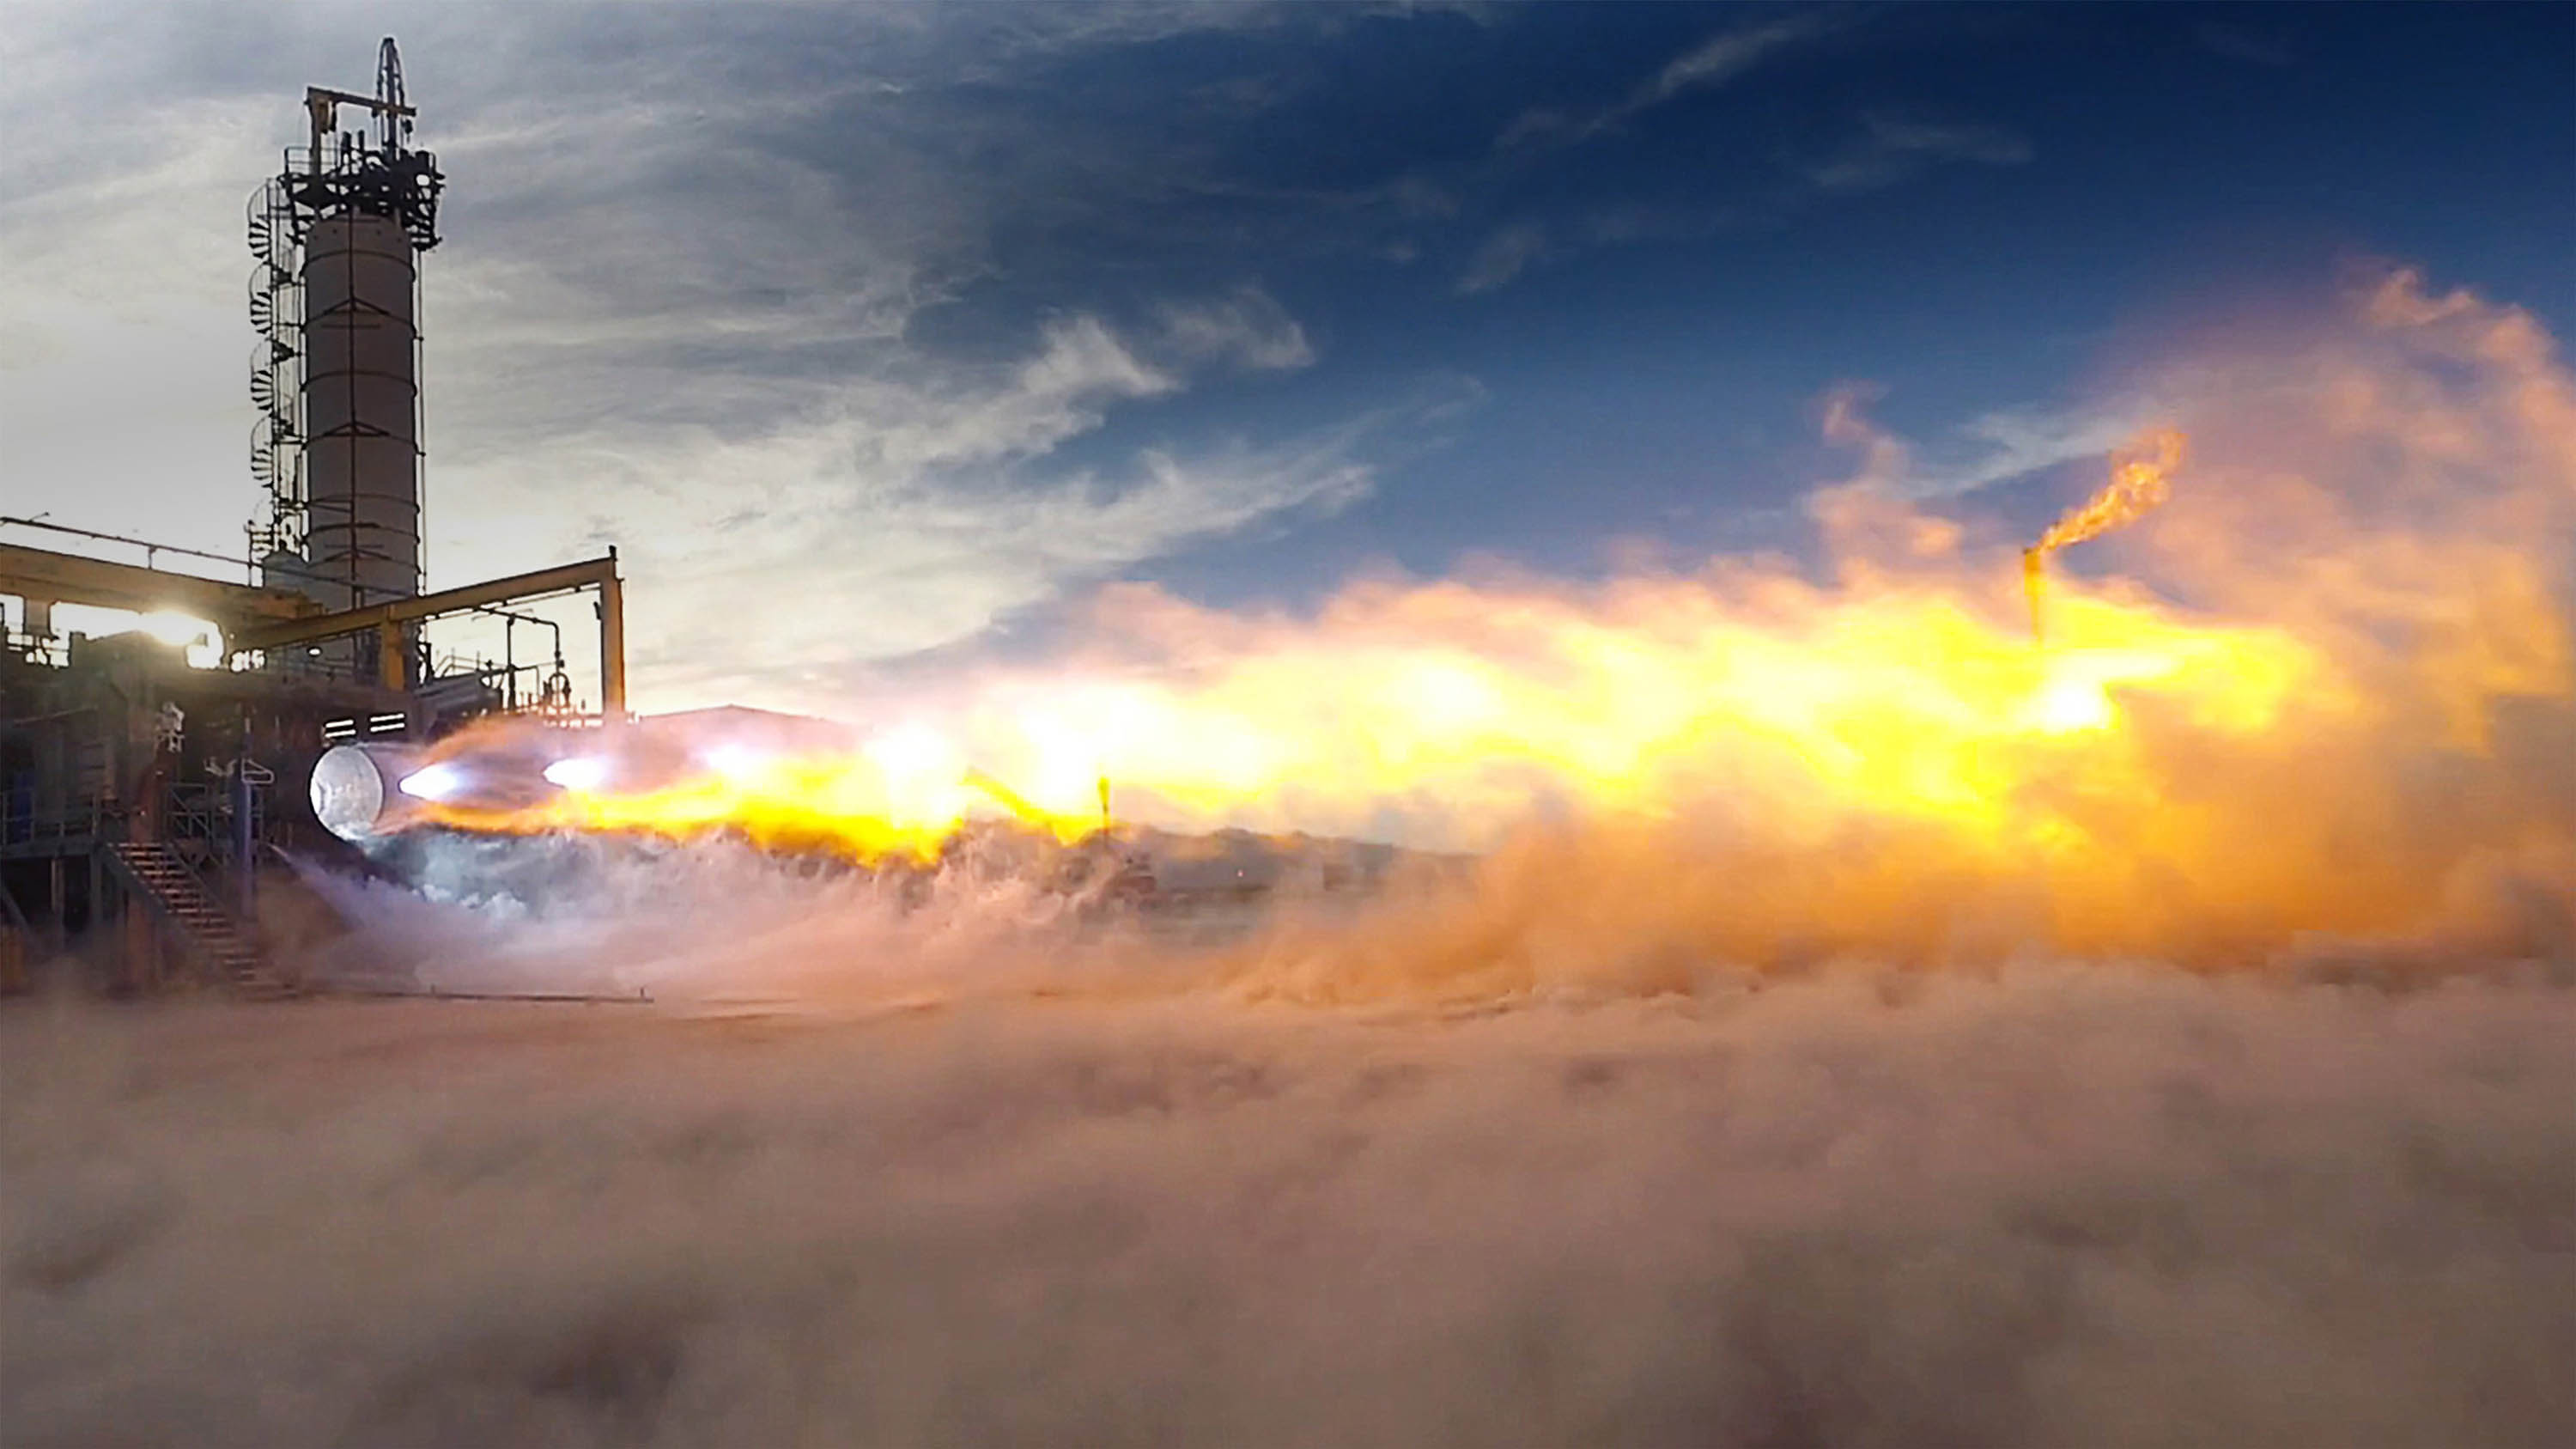
\includegraphics[width=0.99\linewidth]{intro/be4.jpg}
			\caption*{\tiny{Blue Origin, 2018}}
		\end{figure}
	\end{minipage}
	\begin{minipage}{0.33\linewidth}
		\begin{figure}
			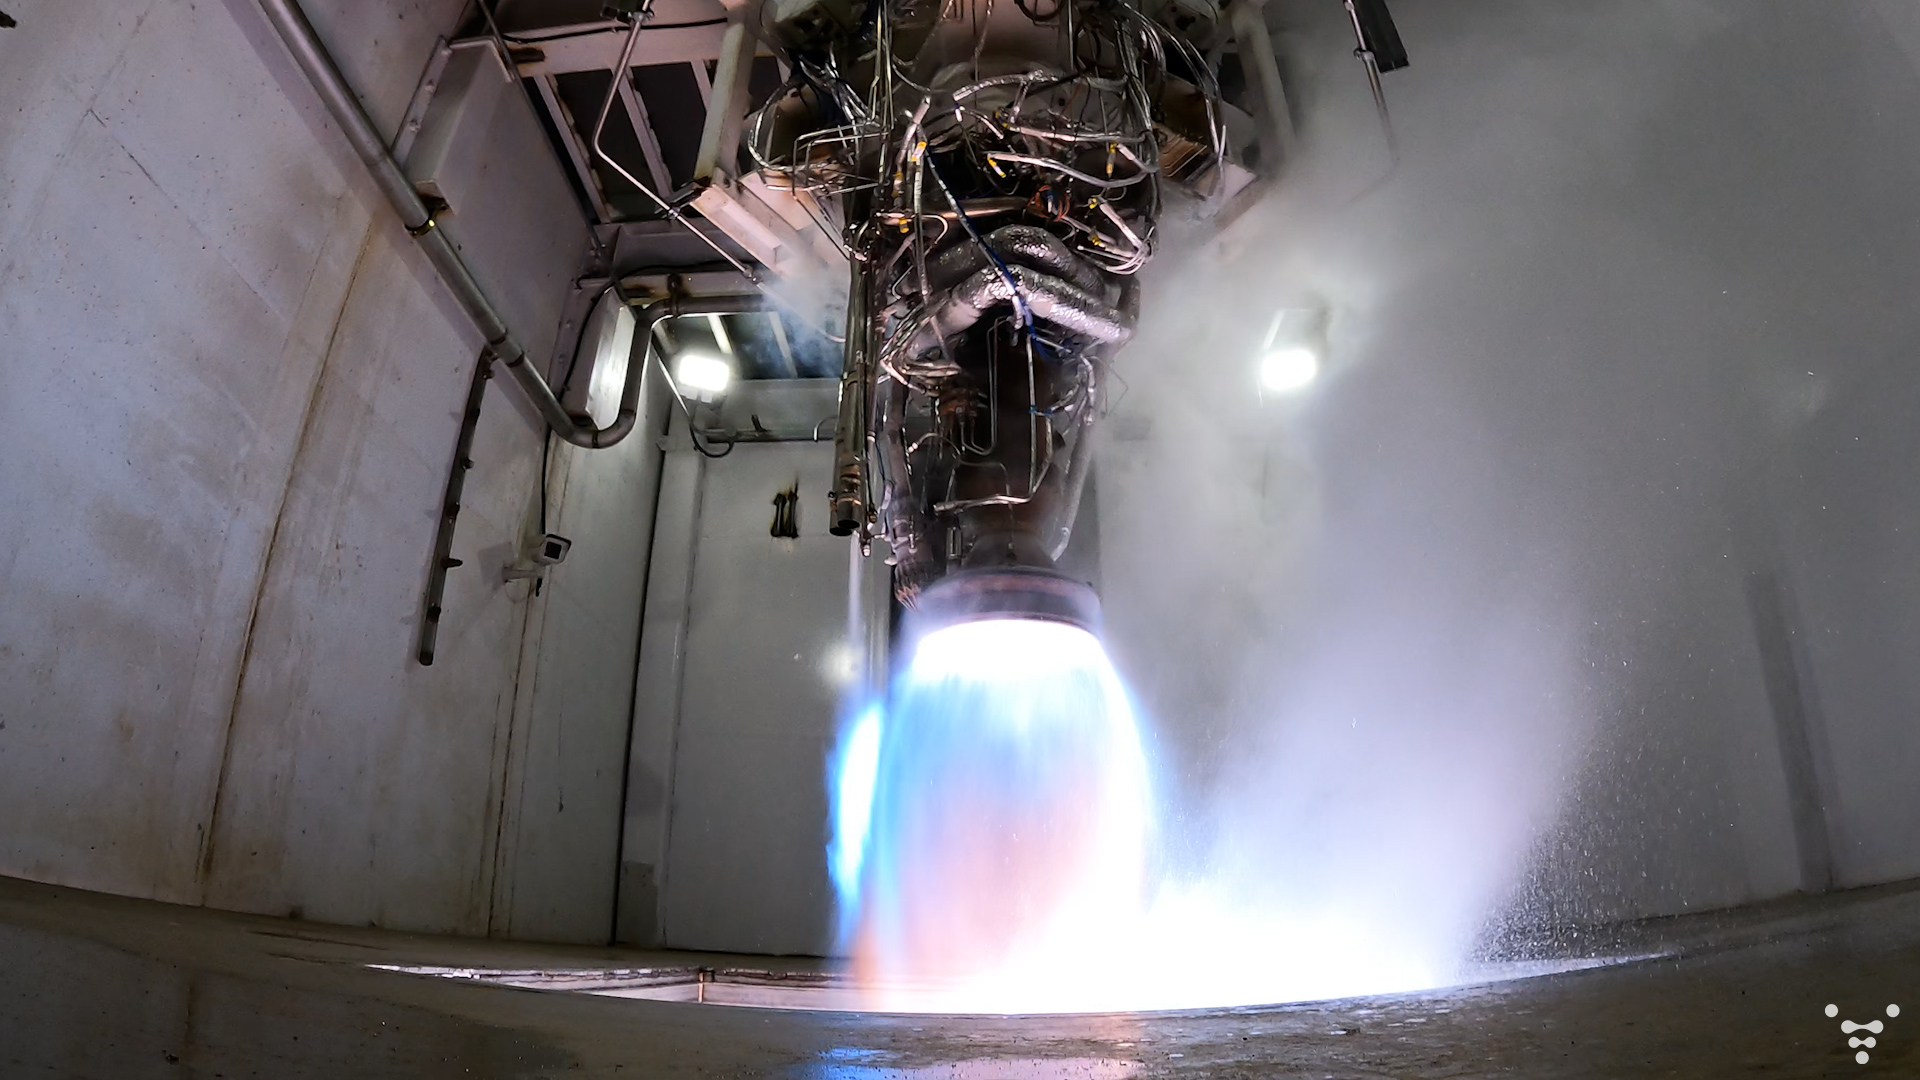
\includegraphics[width=0.99\linewidth]{intro/aeonR.png}
			\caption*{\tiny{Relativity Space, 2022}}
		\end{figure}
	\end{minipage}
	\begin{minipage}{0.28\linewidth}
		\begin{figure}
			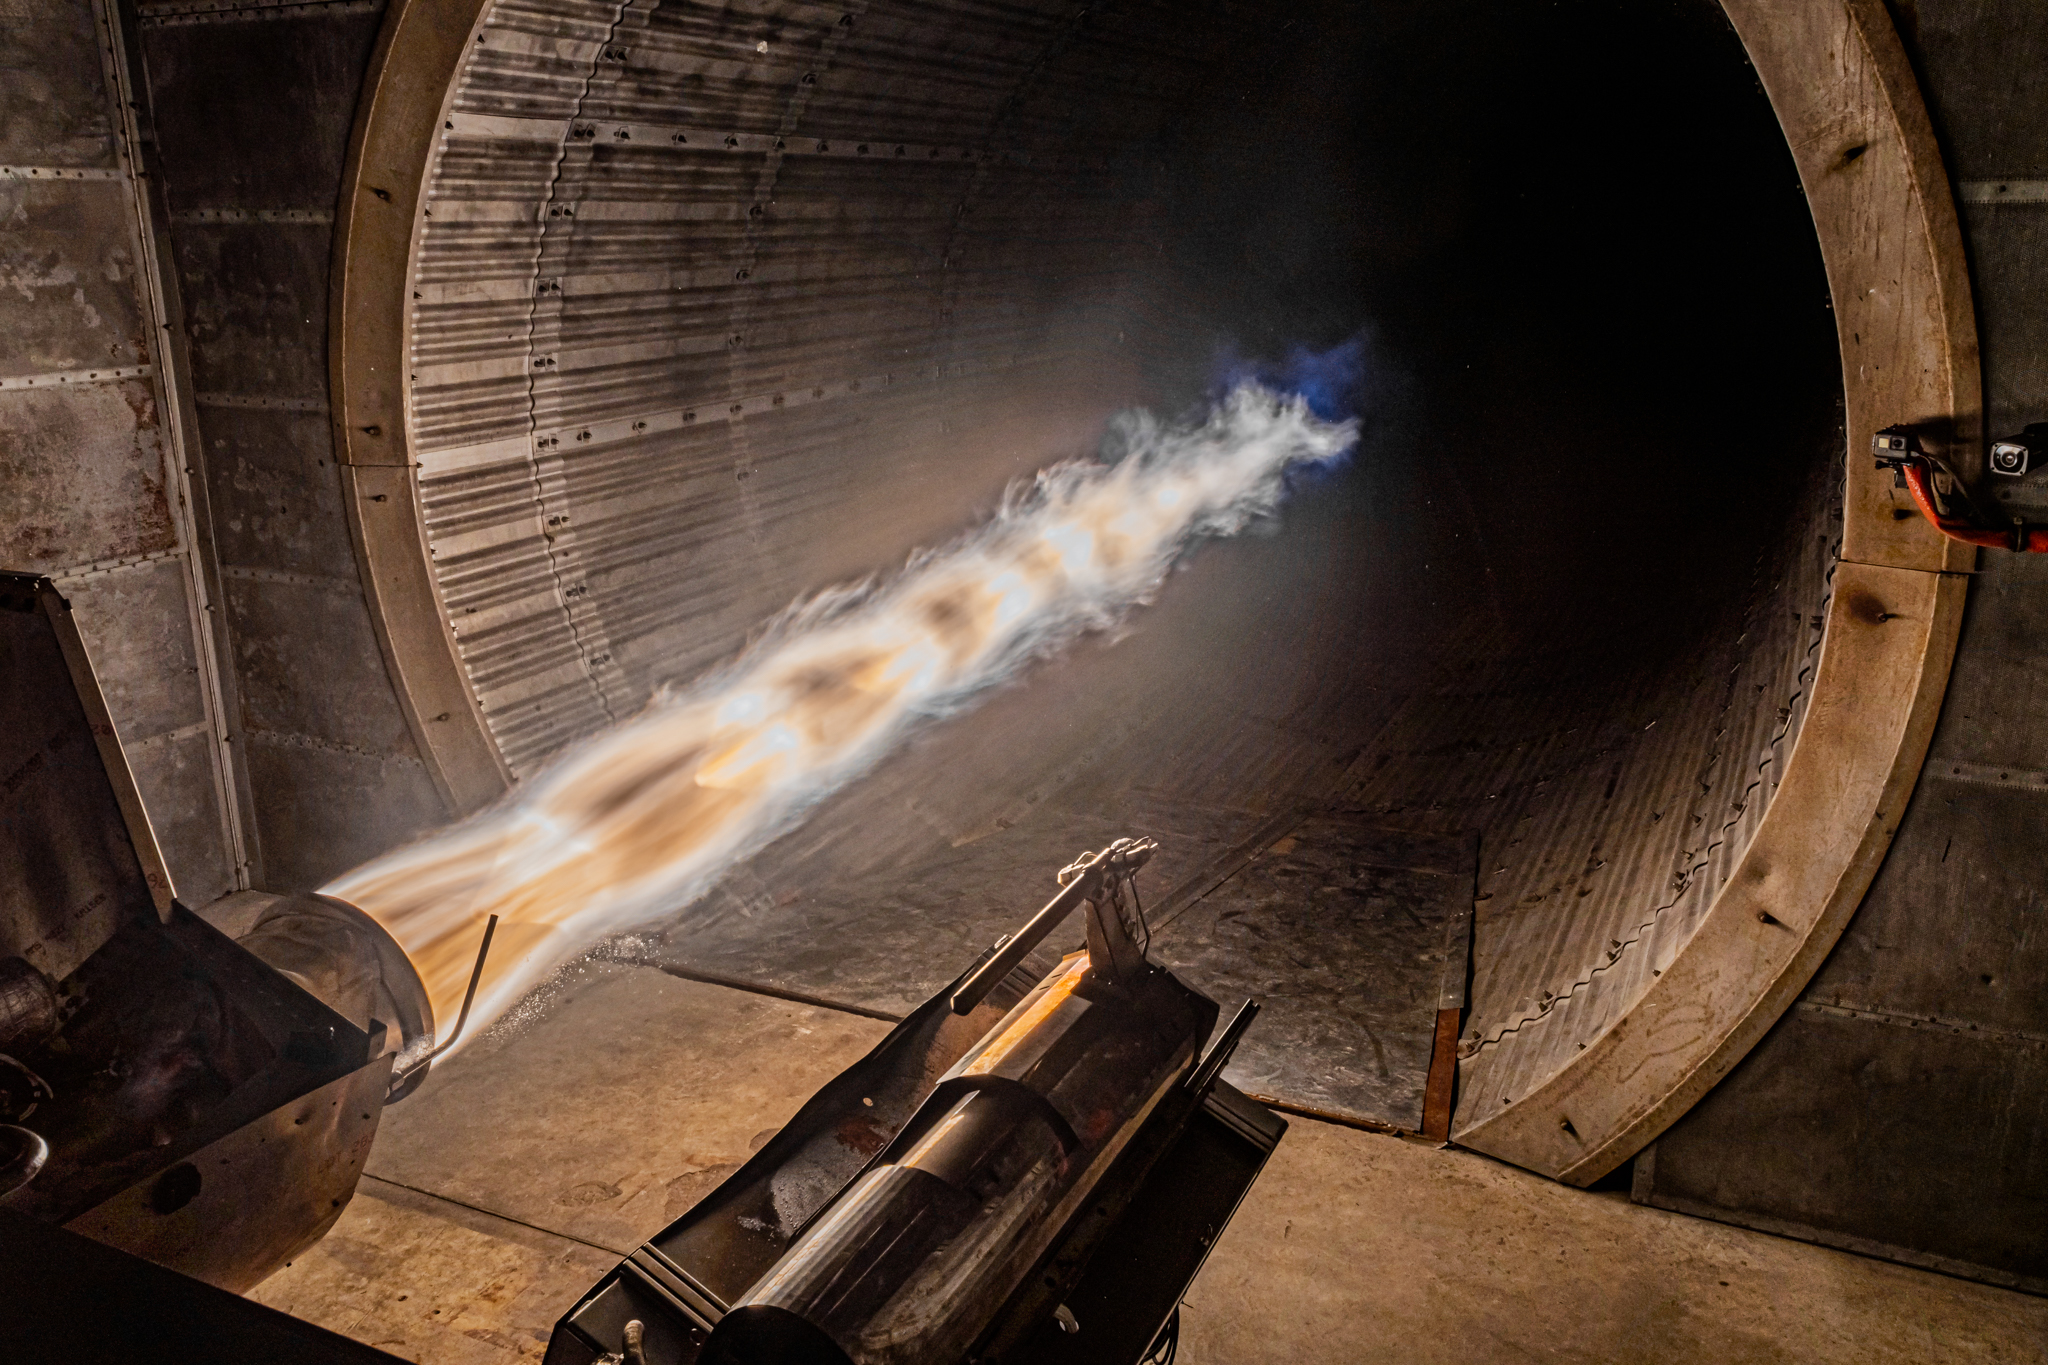
\includegraphics[width=0.99\linewidth]{intro/delphin.jpeg}
			\caption*{\tiny{John Kraus, 2021}}
		\end{figure}
	\end{minipage}
\end{frame}

\begin{frame}{Cost of experiments (in 2022 USD)}
    \begin{itemize}
        \item Rocketdyne F-1 (Saturn V)
        \begin{itemize}
            \item \$4.8 billion development cost
            \item \$30 million per unit
            \item \$1.6 billion per launch
        \end{itemize}
        \item SpaceX Merlin 1D (Falcon Heavy)
        \begin{itemize}
            \item \$1 million per unit
            \item \$97 million per launch
        \end{itemize}
    \end{itemize}
	\begin{minipage}{0.49\linewidth}
		\begin{figure}
			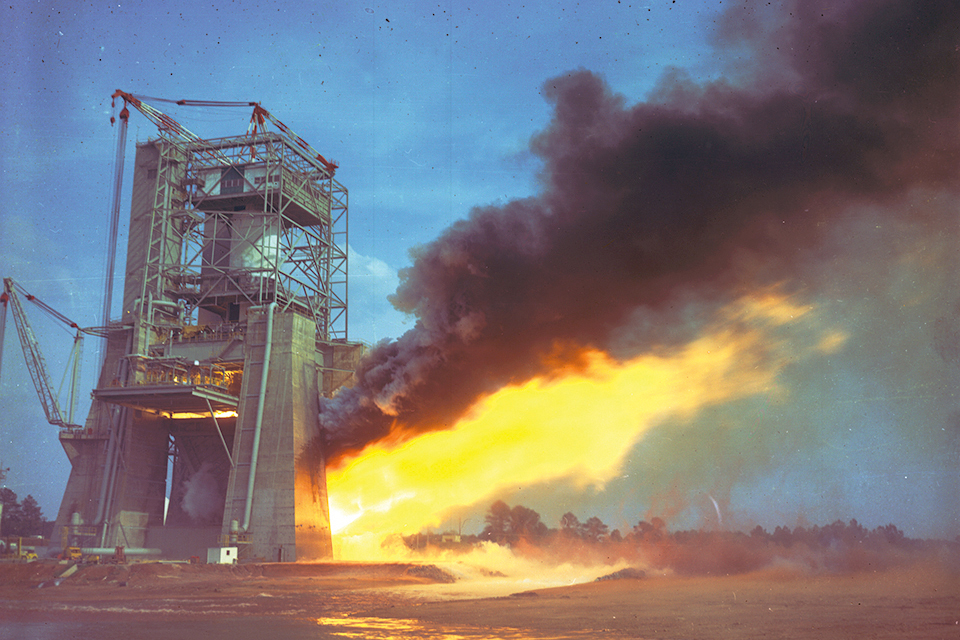
\includegraphics[width=0.9\linewidth]{intro/f1TestStand.jpg}
			\caption*{\tiny{NASA, 1966}}
		\end{figure}
	\end{minipage}
	\begin{minipage}{0.49\linewidth}
		\begin{figure}
			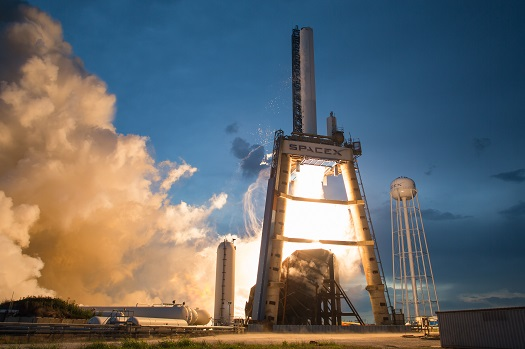
\includegraphics[width=0.9\linewidth]{intro/merlin1dTestStand.jpg}
			\caption*{\tiny{SpaceX, 2013}}
		\end{figure}
	\end{minipage}
\end{frame}

\begin{frame}{Cost of simulations}
    \begin{itemize}
        \item IBM Summit at ORNL
        \begin{itemize}
            \item $\sim$\$200 million (2019 USD) to design and build
            \item 13 MW peak consumption ($\sim$11,000 homes)
            \item $\sim$\$10 million annual energy cost (overestimated)
        \end{itemize}
        \item Combustion LES/DNS
        \begin{itemize}
			\item Years to develop/validate code
            \item $\numDOF \sim \; \text{Re}^{9/4}$
            \item 50+ species, 100+ reactions
            \item $\Delta t = \mathcal{O}(1\text{e-}9 \; s)$
        \end{itemize}
    \end{itemize}
	\centering
	\begin{minipage}{0.3\linewidth}
		\centering
		\begin{figure}
			\centering
			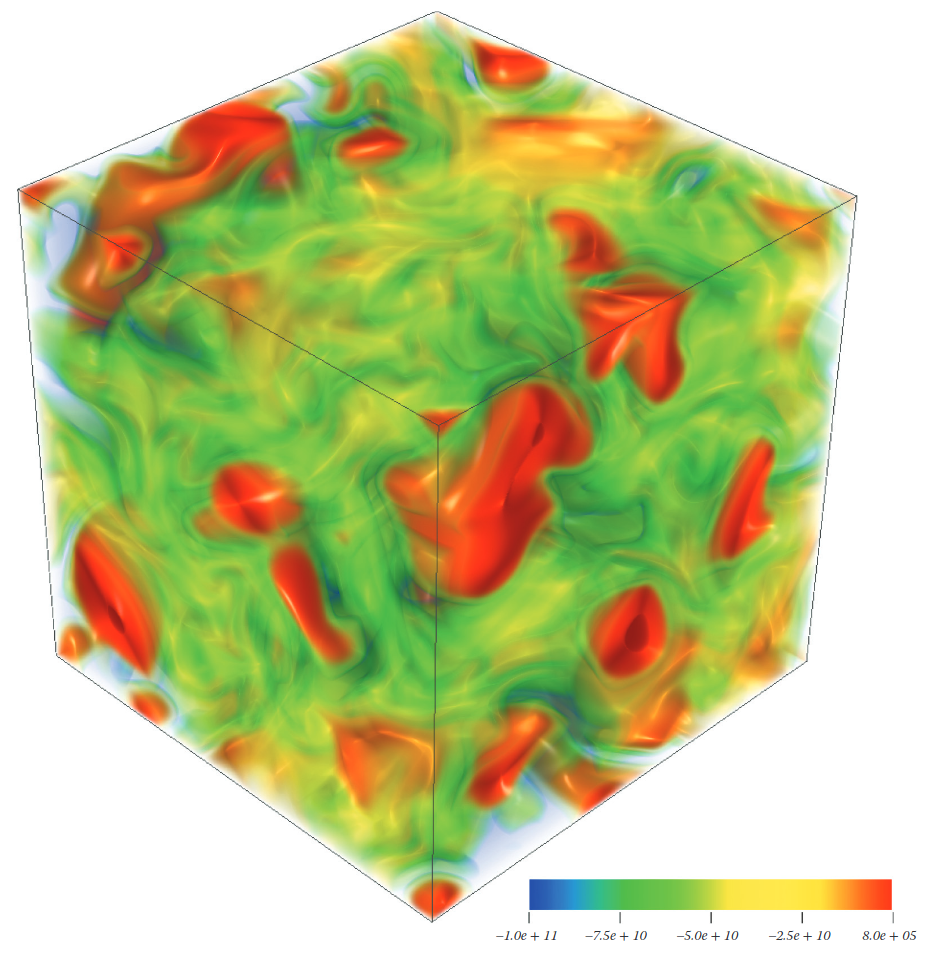
\includegraphics[width=0.87\linewidth]{intro/combustionDNS.png}
			\caption*{\tiny{Treichler et al, 2017}}
		\end{figure}
	\end{minipage}
	\hspace{1cm}
	\centering
	\begin{minipage}{0.3\linewidth}
		\centering
		\begin{figure}
			\centering
			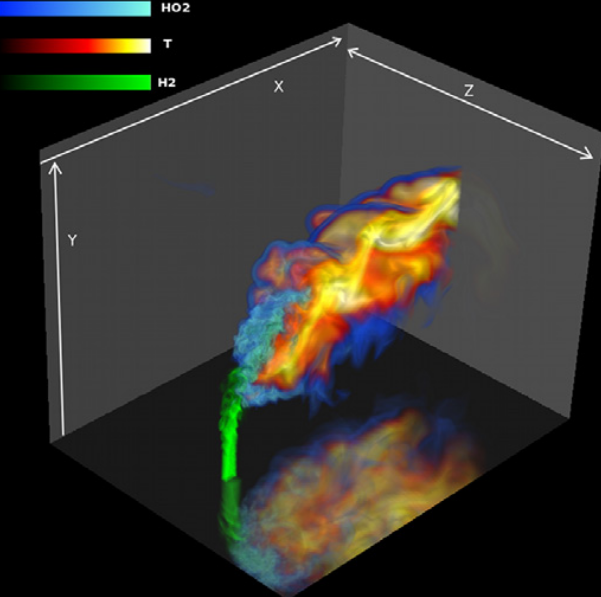
\includegraphics[width=0.91\linewidth]{intro/jetCrossflowDNS.png}
			\caption*{\tiny{Grout et al., 2011}}
		\end{figure}
	\end{minipage}
\end{frame}

\begin{frame}{Data-driven reduced-order models (ROMs)}
	\begin{itemize}
		\item Learning low-cost models from high fidelity simulations, experiments
		\item Evolving \textbf{low-dimensional} state approximation in time
		\item Non-intrusive methods
		\begin{itemize}
			\item Only require system output
			% \item Black/gray box models
			\item Kriging, operator inference, ANNs
		\end{itemize}
		\item Intrusive methods
		\begin{itemize}
			\item Directly manipulate governing equations
			\item Galerkin, Petrov--Galerkin projection
		\end{itemize}
		\item \textbf{Not} reduced-physics models, e.g.
		\begin{itemize}
			\item Reduced chemical mechanisms
			\item Flamelet-progress variable models
			\item Flame transfer functions
		\end{itemize}
	\end{itemize}
\end{frame}

\begin{frame}{Projection-based ROMs (PROMs) of non-linear systems}
    \begin{itemize}
        \item Mapping from low-dim latent space to approximate solution manifold
        \item Map governing equations onto low-dim manifold, evolve in time
    \end{itemize}
	\centering
	\begin{minipage}{0.49\linewidth}
		\centering
		\vspace{-2em}
		\begin{align*}
			\ode{\stateVec}{\timeVar} = \rhsFunc{\stateVec}&, \quad \ode{\stateVecCoef}{\timeVar} = \encoderFunc{\rhsFunc{\decoderFunc{\stateVecCoef}}} \\[1em]
			\stateVec \in \mathbb{R}^{\numDOF}&, \quad \stateVecCoef \in \mathbb{R}^{K} \\[1em]
			\numDOF &\gg K
		\end{align*}
	\end{minipage}
	\hspace{-2em}
	\begin{minipage}{0.49\linewidth}
		\begin{figure}
			\only<1>{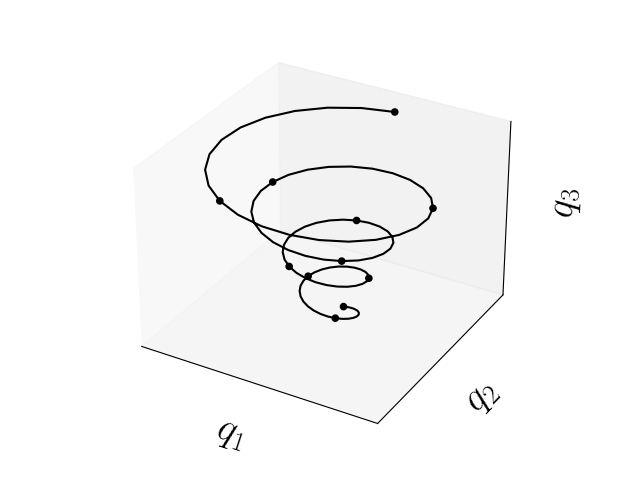
\includegraphics[width=0.9\linewidth]{Images/theory/mapExample_3d.png}}
			\only<2>{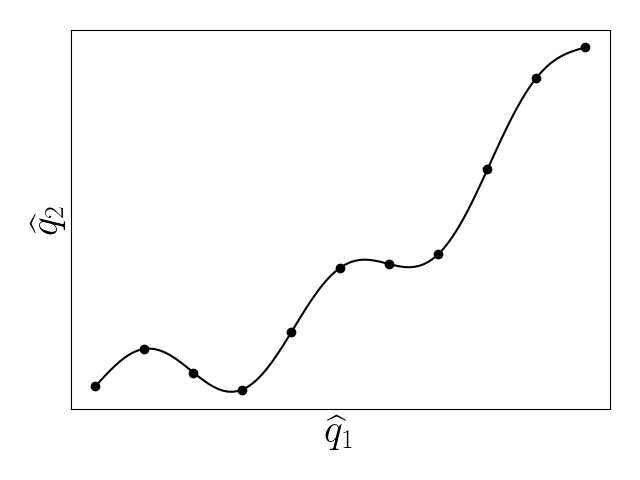
\includegraphics[width=0.9\linewidth]{Images/theory/mapExample_2d.png}}
		\end{figure}
	\end{minipage}
	\begin{tcolorbox}[colframe=blue!50!white,halign=center]
		PROMs of non-linear systems have \textbf{no stability guarantees}
	\end{tcolorbox}
\end{frame}

\begin{frame}{Prior work}
	\begin{itemize}
		\item 2000's
		\begin{itemize}
			\item Balanced truncation, balanced POD (Willcox, Benner) 
			\item Galerkin PROMs for fluid flows (Rowley, Bui-Thanh)
		\end{itemize}
		\item 2010's
		\begin{itemize}
			\item Least-squares Petrov--Galerkin PROMs (Carlberg, Farhat)
			\item MPE, DEIM, GNAT (Willcox, Chaturantabut, Carlberg)
			\item Closure and stabilization (Tezaur, Iliescu, San, Duraisamy)
			\item Local trial bases, dictionary methods (Amsallem, Zahr)
		\end{itemize}
		\item 2020's
		\begin{itemize}
			\item Non-intrusive ROMs (Willcox, Hesthaven)
			\item Non-linear manifold PROMs (Lee, Choi)
			\item Online basis and sampling adaptation (Peherstorfer, Huang)
		\end{itemize}
		
	\end{itemize}
\end{frame}

\begin{frame}{Objectives}
	\begin{itemize}
		\item How are PROMs best extended to \textbf{reacting flows}?
		\item What methods promote \textbf{accurate} and \textbf{scalable} PROM solutions? 
		\item Can PROMs be truly \textbf{predictive} for large-scale systems?
		\item What \textbf{nuances} does the literature fail to adequately detail?
	\end{itemize}

	\begin{figure}
		\begin{minipage}{0.49\linewidth}
			\animategraphics[autoplay,loop,trim=0.5em 0.5em 0.5em 0.5em,width=0.99\linewidth,every=100]{10}{Images/experiments/cvrc/fom_temp/fig_z_Temperature_}{50000}{55000}

			\animategraphics[autoplay,loop,trim=0.5em 0.5em 0.5em 0.5em,width=0.99\linewidth,every=100]{10}{Images/experiments/cvrc/fom_z/fig_z_Flamelet_Scalar_Mean_}{50000}{55000}
		\end{minipage}
		\begin{minipage}{0.45\linewidth}
			\animategraphics[autoplay,loop,trim=1em 1em 1em 1em,width=0.99\linewidth,every=60]{10}{Images/experiments/9elem/fom_pressure/fig_z_Static_Pressure_}{215000}{218900}
		\end{minipage}
	\end{figure}
\end{frame}

\begin{frame}{Contributions}
    \begin{enumerate}
		\item PERFORM, open-source Python package for rapid prototyping novel ROM methods, challenging benchmarks
		\item Scalable PROM solver in high-performance combustion CFD code
        \item State-of-the-art PROMs for multi-scale, multi-physics flow systems
        \item Analysis of cost and performance of sparse sampling methods
        \item First study of PROMs for 3D multi-injector rocket combustor, containing $>$ 250 million DOFs
        \item Truly predictive PROMs for single-element rocket combutor
        \item Best practices for PROMs of multi-scale systems
    \end{enumerate}
\end{frame}

\section*{PROMs}

\begin{frame}{Projection-based ROMs}
    \begin{itemize}
		\item General non-linear ODE
		\begin{equation*}
			\ode{\consVec}{\timeVar} + \rhsFunc{\consVec} = \zeroVec \quad \consVec \in \mathbb{R}^{\numDOF}
		\end{equation*}
			\item Low-dimensional affine representation ($\numConsModes \ll \numDOF$)
		\begin{align*}
			\consVec(\timeVar) \approx \consVecRom(\timeVar) &\defEq \consVecCent + \consScale \sum^{\numConsModes}_{i=1} \consVarCoef{i}(\timeVar) \consTrialVec{i} \\
			&= \consVecCent + \consScale \consTrial \consVecCoef(\timeVar)
		\end{align*}
		\begin{equation*}
			\consVecCoef \in \mathbb{R}^{\numConsModes}, \; \consTrial \in \mathbb{R}^{\numDOF \times \numConsModes}
		\end{equation*}
		\item Centering profile $\consVecCent$ and scaling matrix $\consScale$ are crucial; more later
		\begin{equation*}
			\consScale \defEq \text{diag}\left( \consScaleVar{1}, \; \consScaleVar{2}, \; \hdots \;, \; \consScaleVar{\numDOF} \right)
		\end{equation*}
	\end{itemize}
\end{frame}

\begin{frame}{Linear trial space}
    \begin{itemize}
        \item The proper orthogonal decomposition (POD)\footnotemark[1]
        \begin{equation*}
            \consTrial = \argmin{\dummyMatOne \in \mathbb{R}^{\numDOF \times \numConsModes}} \norm{\consDataMat - \dummyMatOne \dummyMatOne^\top \consDataMat}_2^2
        \end{equation*}
        \begin{equation*}
            \consDataMat = \basisMat \singVecMat \rightSingVecMat^\top, \quad \consTrial \leftarrow \basisMat[:, {:}\numConsModes]
        \end{equation*}
    \end{itemize}
	\centering
	\vspace{-0.8em}
	\begin{figure}
		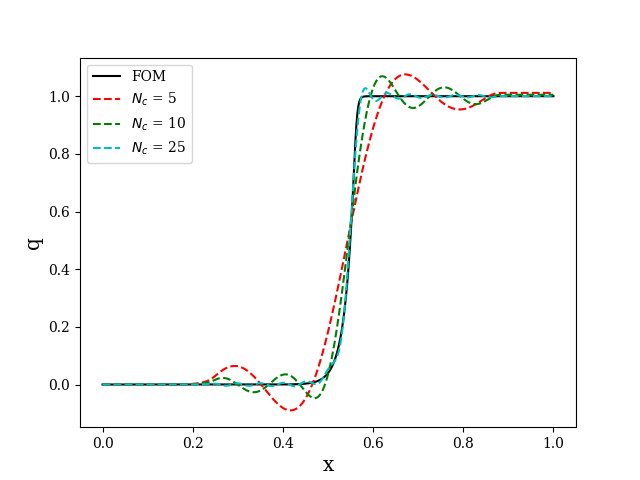
\includegraphics[width=0.5\linewidth]{theory/podProfileConverge.png}
	\end{figure}
	\footnotetext[1]{\tiny{Berkooz et al., \textit{Annu Rev Fluid Mech}, Vol. 25, 1993.}}
\end{frame}

\begin{frame}{The test basis}
    \begin{itemize}
        \item Inserting approximation, no order reduction yet
        \begin{equation*}
            \resScaleInv \left[\consScale \consTrial \ode{\consVecCoef}{\timeVar} + \rhsFunc{\consVecCent + \consScale \consTrial \consVecCoef}\right] = \zeroVec 
        \end{equation*}
        \item Project via test basis $\testBasis \in \mathbb{R}^{\numDOF \times \numConsModes}$, rearrange
        \begin{equation*}
            \ode{\consVecCoef}{\timeVar} + \left[ \testBasis^\top \resScaleInv \consScale \consTrial \right]^{-1} \testBasis^\top \resScaleInv \rhsFunc{\consVecRom} = \zeroVec
        \end{equation*}
        \item $\testBasis = \consTrial$: Galerkin projection
        \item $\testBasis \neq \consTrial$: Petrov--Galerkin projection 
    \end{itemize}
\end{frame}

\begin{frame}{Least-squares Petrov--Galerkin (LSPG)}
	\small
    \begin{itemize}
		\item Fully-discrete residual (e.g. BDF1)
		\begin{equation*}
			\resFuncIter{\timeIdx}{\consVecCoef^{\newtonIdx}} \defEq \consScale \consTrial \left( \consVecCoef^{\newtonIdx} - \consVecCoef^{\timeIdx-1} \right) + \dt \, \rhsFunc{\consVecCent + \consScale \consTrial \consVecCoef^{\newtonIdx}} = \zeroVec
		\end{equation*}
		\item Minimize with Gauss--Newton
		\begin{equation*}
			\delta \consVecCoef^{\newtonIdx, \timeIdx} = \argmin{\dummyVec \in \mathbb{R}^{\numConsModes}} \norm{\resScaleInv \left(\pde{\resFuncIter{\timeIdx}{\dummyVec}}{\dummyVec} \dummyVec + \resFuncIter{\timeIdx}{\dummyVec}\right)}_2^2
		\end{equation*}
		\item Equivalent to Petrov--Galerkin projection with test basis\footnotemark[2]
		\begin{equation*}
			\testBasis = \resScaleInv \pde{\resFuncIter{\timeIdx}{\consVecCoef^{\newtonIdx}}}{\consVec} \consScale \consTrial, \quad 
		\end{equation*}
		\vspace{-2em}
		\item Stable for LTI systems
		\begin{equation*}
			\left\Vert \left(\testBasis^\top \testBasis\right)^{-1} \testBasis \consTrial \right\Vert_2 \le \frac{1}{\sigma_{\numConsModes}\left(\testBasis\right)}, \quad \sigma_{\numConsModes}\left(\testBasis\right) \ge \sigma_{\numDOF}\left(\mathbf{A}\right) \ge 1 
		\end{equation*}
	\end{itemize}
	\vspace{-1em}
	\begin{tcolorbox}[colframe=blue!50!white,halign=center]
		LSPG is \textbf{discrete-optimal} at every time step
	\end{tcolorbox}
	\normalsize
	\footnotetext[2]{\tiny{Carlberg el al., \textit{Int. J. Numer. Meth. Engng}, Vol. 86, 2010.}}
\end{frame}

\begin{frame}{State of the art in 2017}
	\begin{itemize}
		\item PROMs for parametrized elliptic problems are extremely robust\footnotemark[3]
		\item Galerkin ROMs are generally unstable for unsteady problems
		\item LSPG is leap forward, biggest case in 3D Ahmed body\footnotemark[4]
		\item First studies of PROMs for reacting flows suffer from instabilities\footnotemark[5]
	\end{itemize}
	
	\begin{minipage}{0.4\linewidth}
		\begin{figure}
			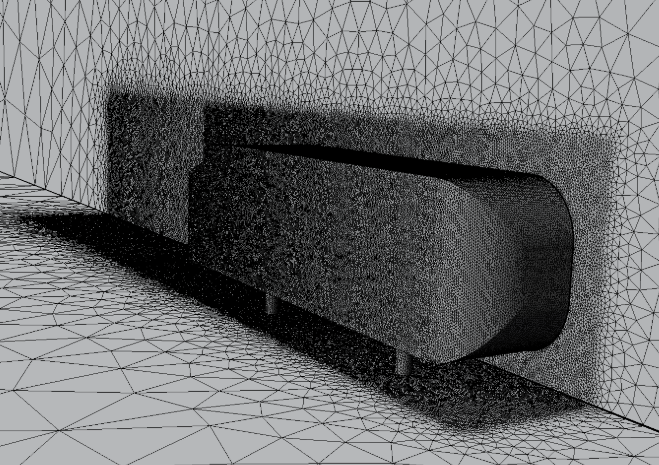
\includegraphics[width=0.99\linewidth]{theory/ahmed.png}
			\caption*{\tiny{Carlberg et al., 2013}}
		\end{figure}
	\end{minipage}
	\begin{minipage}{0.58\linewidth}
		\begin{figure}
			\animategraphics[autoplay,loop,trim=1em 1em 1em 1em,width=0.99\linewidth]{10}{theory/single_injector/fom/fig_}{00000}{00046}
			\animategraphics[autoplay,loop,trim=1em 1em 1em 1em,width=0.99\linewidth]{10}{theory/single_injector/rom/fig_}{00000}{00046}
			\caption*{\tiny{Huang, 2018}}
		\end{figure}
	\end{minipage}

	\footnotetext[3]{\tiny{Hesthaven et al., \textit{Certified Reduced Basis Methods for Parametrized Partial Differential Equations}, Springer, 2015.}}
	\footnotetext[4]{\tiny{Carlberg et al., \textit{J Comp Phys}, Vol. 242, 2013.}}
	\footnotetext[5]{\tiny{Huang et al., \textit{AIAA Propulsion and Energy}, 2018.}}
\end{frame}

\section*{MP-LSVT}

\begin{frame}{Generalizing least-squares ROMs}
    \begin{itemize}
		\item LSPG trial space formulated for the conserved variables, but \textbf{alternative variables} can prove useful
		\begin{itemize}
			\item Entropy variables
			\item Quadratic lifting variables
		\end{itemize}
		\item Choose \textbf{any} complete set of variables, e.g. primitive variables
		\begin{equation*}
			\stateVar_p \defEq \left[ p, \; u_i, \; T, \; Y_l \right]
		\end{equation*}
		\item Construct linear approximation, supply mapping to conserved variables
		\begin{equation*}
			\primVecRom(\timeVar) \defEq \primVecCent + \primScale \primTrial \primVecCoef(\timeVar), \quad \primVecCoef \inROne{\numPrimModes}
		\end{equation*}
		\begin{equation*}
			\consVec \defEq \consVec \left( \primVecRom \right)
		\end{equation*}
	\end{itemize}
\end{frame}

\begin{frame}{\small{Model-form preserving least-squares with variable transformation (MP-LSVT)}}
	\begin{itemize}
		\item Frame residual in terms of target state\footnotemark[6]
		\begin{equation*}
			\resFuncIter{\timeIdx}{\primVecCoef^{\newtonIdx}} \defEq \consFunc{\primVecCent + \primScale \primTrial \primVecCoef^{\newtonIdx}} - \consVec^{\timeIdx-1} + \dt \, \rhsFunc{\primVecCent + \primScale \primTrial \primVecCoef^{\newtonIdx}} = \zeroVec
		\end{equation*}
		\item Gauss--Newton w/r/t \textbf{target variable} modal coefficients
		\begin{equation*}
			\testBasis = \resScaleInv \pde{\resFuncIter{\timeIdx}{\primVecCoef^{\newtonIdx}}}{\primVec} \primScale \primTrial
		\end{equation*}
	\end{itemize}
	\begin{minipage}{0.4\linewidth}
		\centering
		\begin{figure}
			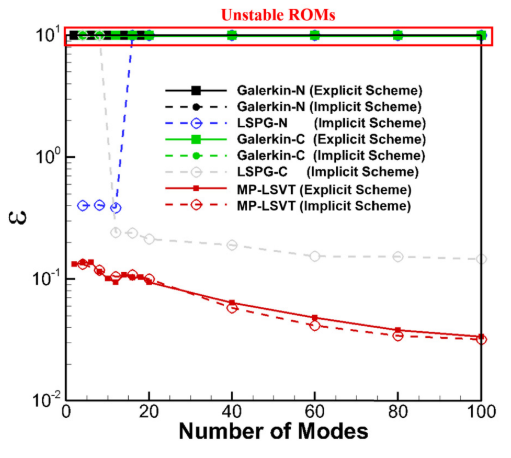
\includegraphics[width=0.9\linewidth]{theory/mplsvt_err_vs_modes.png}
		\end{figure}
	\end{minipage}
	\begin{minipage}{0.58\linewidth}
		\begin{tcolorbox}[colframe=blue!50!white,halign=center]
			Enhances accuracy and conditioning for \textbf{extremely stiff} systems
		\end{tcolorbox}
	\end{minipage}
	\footnotetext[6]{\tiny{Huang, \textbf{Wentland}, and Duraisamy, \textit{J Comp Phys.}, Vol. 448, 2022.}}
\end{frame}

\section*{Hyper-reduction}

\begin{frame}{The lifting bottleneck}
    \begin{itemize}
		\item Non-linear terms $\rhsFunc{\primVecRom}$ still scale with full dimension $\numDOF$
		\item For same time integrator and \dt, ROM is usually \textbf{more} expensive
		\item Can we approximate non-linear terms from a few samples?
		\begin{equation*}
			\rhsFunc{\primVec} \approx \sampFunc{\sampMat \rhsFunc{\primVec}}, \quad \sampMat \in \mathbb{R}^{\numSamps \times \numDOF}
		\end{equation*}
	\end{itemize}
	\vspace{1em}
	\begin{figure}
		\centering
		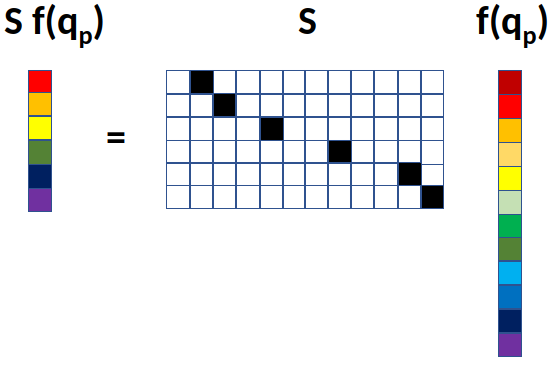
\includegraphics[width=0.55\linewidth]{theory/samplingHelperVis.png}
	\end{figure}
\end{frame}

\begin{frame}{Hyper-reduction by gappy POD}
    \begin{itemize}
		\item Approximate non-linear terms with POD basis $\deimBasis \in \mathbb{R}^{\numDOF \times \numResModes}$, sample
		\begin{equation*}
			\sampMat \resApproxFunc{\primVecCoef} = \sampMat \deimBasis \dummyVec
		\end{equation*}
		\item Least-squares regression, gappy POD\footnotemark[7] ($\numSamps > \numResModes$)
		\begin{equation*}
			\resApproxFunc{\primVecCoef} \defEq \deimBasis \left[ \sampMat \deimBasis \right]^{+} \sampMat \resFunc{\primVecCoef}
		\end{equation*}
		\item MP-LSVT hyper-reduced PROM (HPROM)
		\begin{equation*}
			\left[ \testBasis^\newtonIdx \right]^\top \testBasis^\newtonIdx \delta \primVecCoef^{\newtonIdx} = -\left[\testBasis^\newtonIdx \right]^\top \deimBasis \left[ \sampMat \deimBasis \right]^{+} \sampMat \resScaleInv \resFunc{\primVecCoef^{\newtonIdx}}
		\end{equation*}
		\begin{equation*}
			\testBasis^\newtonIdx \defEq \deimBasis \left[ \sampMat \deimBasis \right]^{+} \sampMat \resScaleInv \jacobResPrim^{\newtonIdx} \primTrial
		\end{equation*}
	\end{itemize}
	\begin{tcolorbox}[colframe=blue!50!white,halign=left]
		PROM: \; $8 \mathbf{\numDOF} \omega + 4 \mathbf{\numDOF} \numPrimModes^2 + 14 \mathbf{\numDOF} \numPrimModes + \numPrimModes^3 - \numPrimModes^2$ \\
		HPROM: $8 \mathbf{\numSamps} \omega + 4 \mathbf{\numSamps} \numPrimModes^2 + 14 \mathbf{\numSamps} \numPrimModes + 2 \mathbf{\numSamps} \numResModes \numPrimModes + \mathbf{\numSamps} \numResModes - \numResModes + \numPrimModes^3 - \numPrimModes^2$
	\end{tcolorbox}
	\footnotetext[7]{\tiny{Everson and Sirovich, \textit{J Opt Soc Am A}, Vol. 12 (8), 1995, pp 1657--1664.}}
\end{frame}

\begin{frame}{Parallel scalability}
	\begin{itemize}
		\item Only need mesh elements required for $\sampMat \resFunc{\consVec} = \resFunc{\sampMatFull \consVec}$
		\item ``Sample mesh'' consumes a fraction of FOM memory
		\item Careful partitioning eliminates MPI communications
	\end{itemize}
	\begin{figure}
		\centering
		\begin{minipage}{0.4\linewidth}
			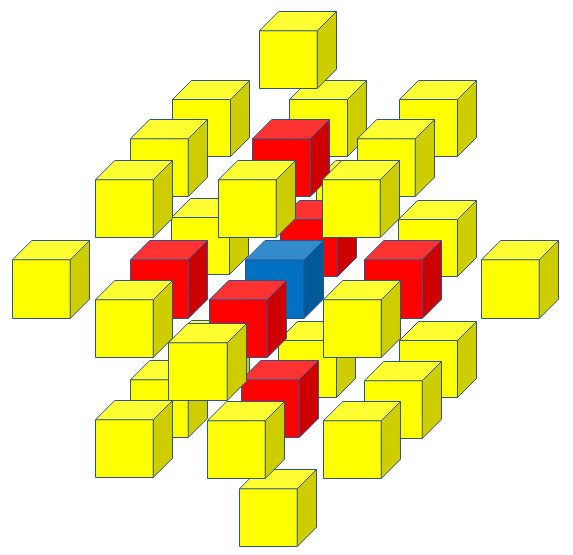
\includegraphics[width=0.9\linewidth]{Images/theory/sampling_3d_2ndOrder.png}
		\end{minipage}
		\begin{minipage}{0.4\linewidth}
			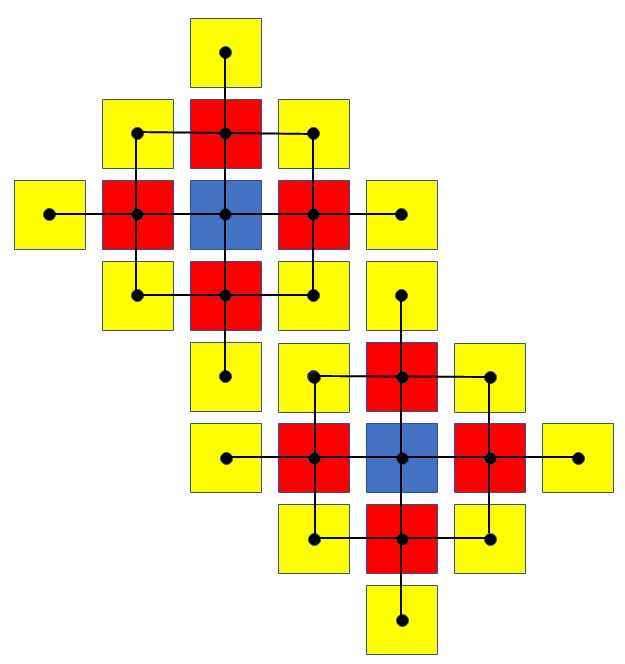
\includegraphics[width=0.8\linewidth]{Images/theory/load_balancing_withEdgeCuts_noSyms.png}
		\end{minipage}
	\end{figure}
	\begin{tcolorbox}[colframe=blue!50!white,halign=center]
		HPROM is \textbf{independent} of full-order dimension $\numDOF$ \\
		Enables computations on \textbf{laptops/workstations} 
	\end{tcolorbox}
\end{frame}

\begin{frame}{Sampling algorithms}
    \begin{itemize}
		\item Computing optimal sampling $\sampMat$ is intractable
		\item Usually resort to greedy (locally-optimal) algorithms
		\begin{itemize}
			\item GNAT (two variants)$^{5,8}$
			\item Eigenvector-based\footnotemark[8]
		\end{itemize}
	\end{itemize}
	\vspace{-1em}
	\begin{minipage}{0.13\linewidth}
		\footnotesize
		\vspace{3.9em}
		\textbf{Random}
		\normalsize

		\vspace{3em}

		\footnotesize
		\textbf{GNAT}

		\vspace{3.7em}

		\footnotesize
		\textbf{Eigenvec}

		\vspace{4em}
	\end{minipage}
	\centering
	\begin{minipage}{0.8\linewidth}
		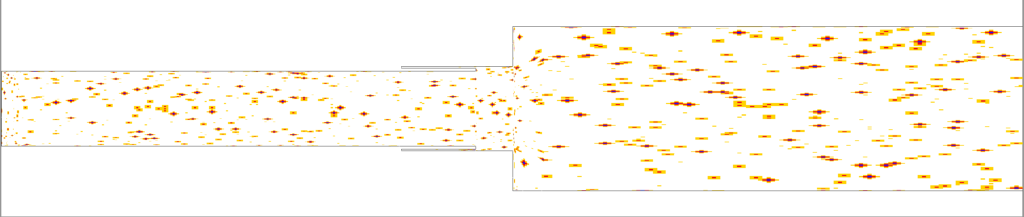
\includegraphics[width=0.85\linewidth,trim={0.2em 2em 0.3em 2em},clip]{Images/theory/iblanks/random_iblank_z.png}

		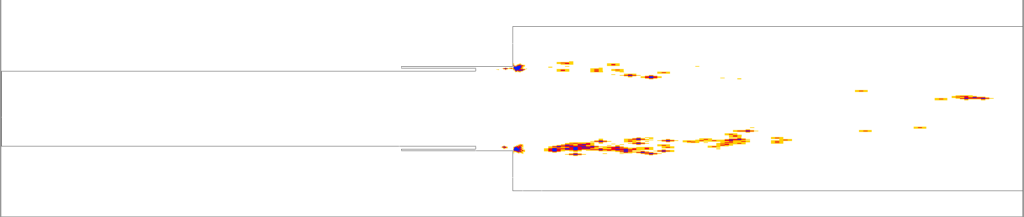
\includegraphics[width=0.85\linewidth,trim={0.2em 2em 0.3em 2em},clip]{Images/theory/iblanks/greedy_ben_iblank_z.png}

		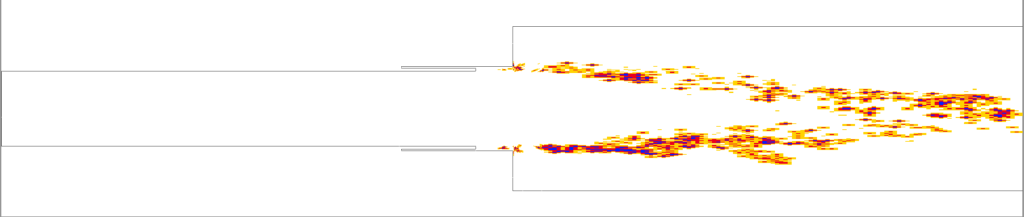
\includegraphics[width=0.85\linewidth,trim={0.2em 2em 0.3em 2em},clip]{Images/theory/iblanks/eigenvec_iblank_z.png}
	\end{minipage}
	\vspace{-2em}
	\footnotetext[8]{\tiny{Peherstorfer et al., \textit{SIAM J Comp Sci}, Vol. 42, 2020.}}
\end{frame}

\begin{frame}{Methodology review}
	\begin{itemize}
		\item ROMs leverage data to build low-dimensional approximations
		\item Galerkin and LSPG PROMs fail for reacting flows
		\item MP-LSVT PROMs enhance stability and accuracy for stiff systems
		\item Gappy POD enables scalable solutions, unlocks cost savings
		\item Greedy algorithms make principled estimates, but vary greatly
	\end{itemize}
\end{frame}

\section*{}

\begin{frame}{Full-order model}
    \begin{itemize}
		\item Compressible Navier--Stokes equations with scalar transport
		\item 2nd-order unstructured finite volume
		\item BDF2 time integration w/ pseudo time-stepping
		\item Finite-rate and flamelet-progress variable chemistry models
	\end{itemize}
	\begin{equation*}
		\pde{\consVec}{\timeVar} + \nabla \cdot (\invFluxDir - \viscFluxDir) = \sourceVec
	\end{equation*}
	\scriptsize
	\def\arraystretch{2}
	\begin{equation*}
		\consVec = \left[
		\begin{array}{c}
		\rho \\ \rho u \\ \rho v \\ \rho w \\ \rho h^0 - p \\ \hdashline[2pt/2pt] \rho Y_{\specIdx} \\
		\end{array}
		\right]  \; \;
		\invFluxDir = \left[
		\begin{array}{c}
		\rho u_i \\  \rho uu_i + \delta_{xi} p \\ \rho vu_i + \delta_{yi} p \\ \rho wu_i + \delta_{zi} p \\ \rho h^0 u_i \\ \hdashline[2pt/2pt] \rho Y_{\specIdx} u_i 
		\end{array}
		\right]  \; \;
		\viscFluxDir = \left[
		\begin{array}{c}
		0 \\ \tau_{ix} \\ \tau_{iy} \\ \tau_{iz} \\ u_j \tau_{ji} - q_i \\ \hdashline[2pt/2pt] \rho D_\specIdx  \pde{Y_{\specIdx}}{x_i}
		\end{array}
		\right]  \; \;
		\mathbf{s} = \left[
		\begin{array}{c}
		0 \\ 0 \\ 0 \\ 0 \\ 0 \\ \hdashline[2pt/2pt] \dot{\omega}
		\end{array} \right]
	\end{equation*}
	\normalsize
\end{frame}

\section*{PERFORM}

\begin{frame}{\footnotesize{Prototyping Environment for Reacting Flow Order Reduction Methods (PERFORM)}}
	\begin{itemize}
		\small
		\item Open-source 1D reacting flow solver w/ flexible ROM API\footnotemark[9]
		\item Used for linearized ROMs\footnotemark[10], adaptive HPROMs\footnotemark[11], AERO 577 projects
		\normalsize
	\end{itemize}
	\vspace{0.5em}
	\begin{minipage}{0.49\linewidth}
		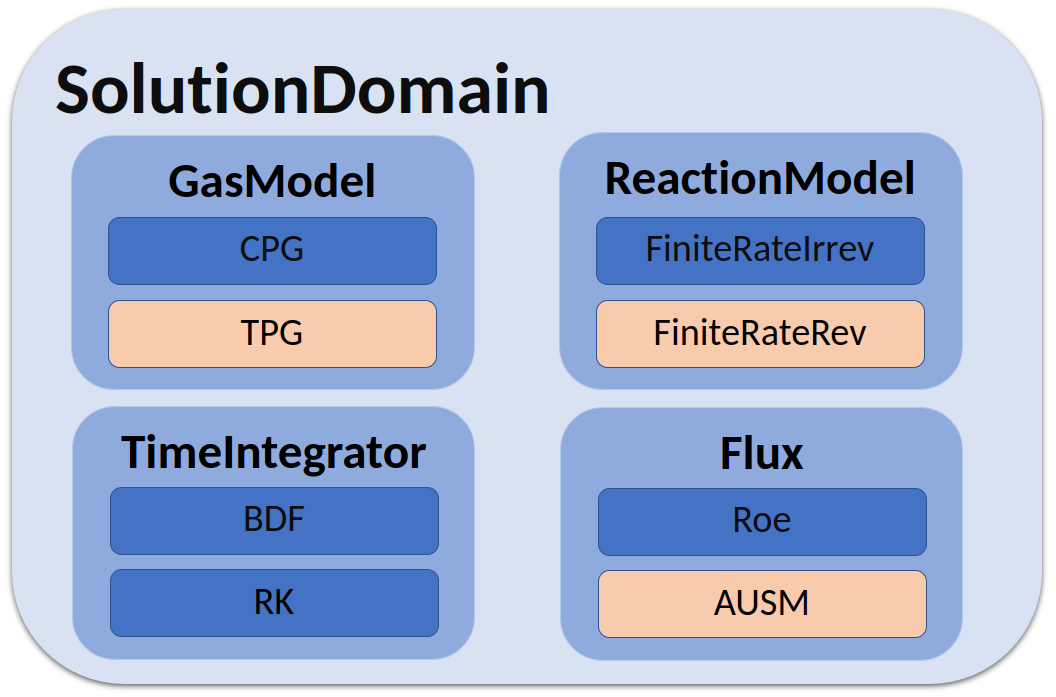
\includegraphics[width=0.99\linewidth]{Images/experiments/transientFlame/performFOMAPI.png}
	\end{minipage}
	\begin{minipage}{0.49\linewidth}
		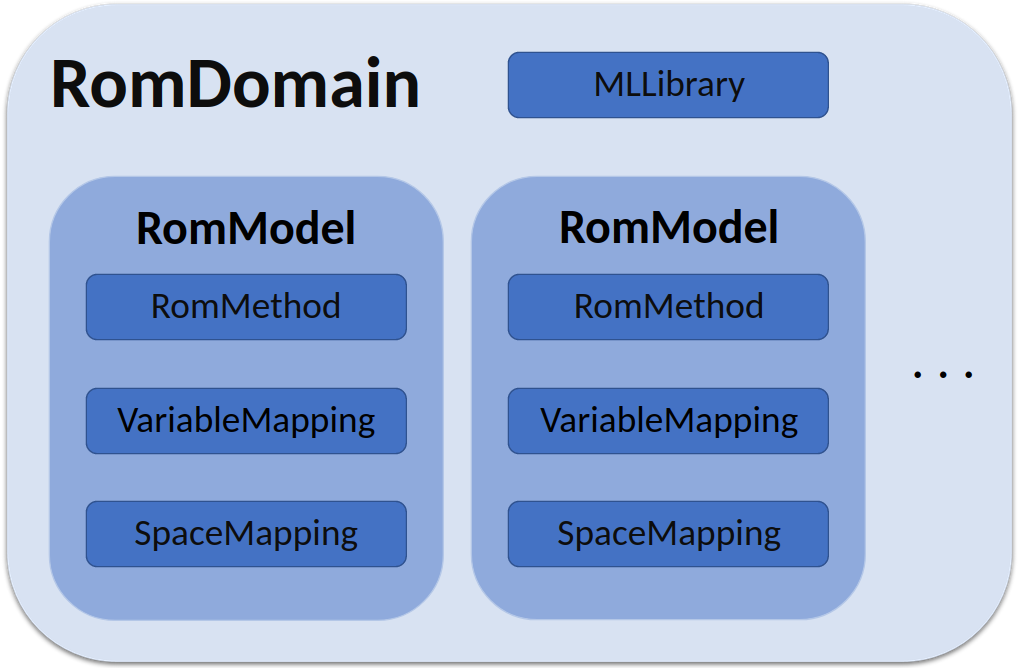
\includegraphics[width=0.99\linewidth]{Images/experiments/transientFlame/performROMAPI.png}
	\end{minipage}

	\vspace{1em}
	\centering
	\texttt{https://github.com/cwentland0/perform}
	\footnotetext[9]{\tiny{\textbf{Wentland} and Duraisamy, \textit{J Open Source Soft.}, 2022.}}
	\footnotetext[10]{\tiny{Rezaian et al., \textit{Phil. Trans. Royal Soc. A}, Vol. 380, 2022.}}
	\footnotetext[11]{\tiny{Uy et al., \textit{arXiv:2209.06957}, 2022.}}
\end{frame}

\begin{frame}{Acoustically-forced model premixed flame}
	\begin{itemize}
		\item Compare linear and non-linear manifold intrusive PROMs, non-intrusive neural network approaches
	\end{itemize}

	\centering
	\begin{figure}
		\animategraphics[controls={play,stop},buttonsize=1em,width=0.59\linewidth,every=1]{5}{Images/experiments/transientFlame/agg/fig_}{1}{50}
	\end{figure}
	
	\begin{tcolorbox}[colframe=blue!50!white,halign=center]
		Explore \textbf{novel} ROMs for \textbf{challenging} benchmark problems
	\end{tcolorbox}
\end{frame}

\section*{Scalable PROMs}

\begin{frame}{HPROMs of multi-scale, multi-physics system}
	\begin{itemize}
		\item HPROMs rarely tested for larger, practical systems
		\item Understanding the effects of:
		\begin{itemize}
			\item Sampling rate $\numSamps$
			\item Gappy POD regressor dimension $\numResModes$
			\item Sampling algorithm
		\end{itemize}
		\item Stability, accuracy, load balancing,computational cost
	\end{itemize}

	\begin{equation*}
		\ell^2\text{-error} = \frac{1}{\numSnaps} \sum_{\timeIdx=1}^{\numSnaps} \frac{\left\Vert \primVec^{\timeIdx} - \primVecRom^{\timeIdx} \right\Vert_2}{\left\Vert \primVec^{\timeIdx} \right\Vert_2}
	\end{equation*}

	\begin{equation*}
		\text{Speedup ratio} = \frac{(\text{FOM wall time}) \times (\text{\# FOM cores})}{(\text{ROM wall time}) \times (\text{\# ROM cores})}
	\end{equation*}
\end{frame}

\begin{frame}{2D transonic flow over an open cavity}
    \begin{itemize}
		\item Ma = 0.6 flow over rectangular cavity\footnotemark[12]
		\item Validation for non-reacting multi-scale system
	\end{itemize}
	\begin{figure}
		\begin{minipage}{0.59\linewidth}
			\animategraphics[autoplay,loop,trim=1em 1em 1em 1em,width=0.99\linewidth,every=50]{10}{Images/experiments/2d_cavity/fom_pressure/fig_Static_Pressure_}{100000}{103000}
		\end{minipage}
		\begin{minipage}{0.4\linewidth}
			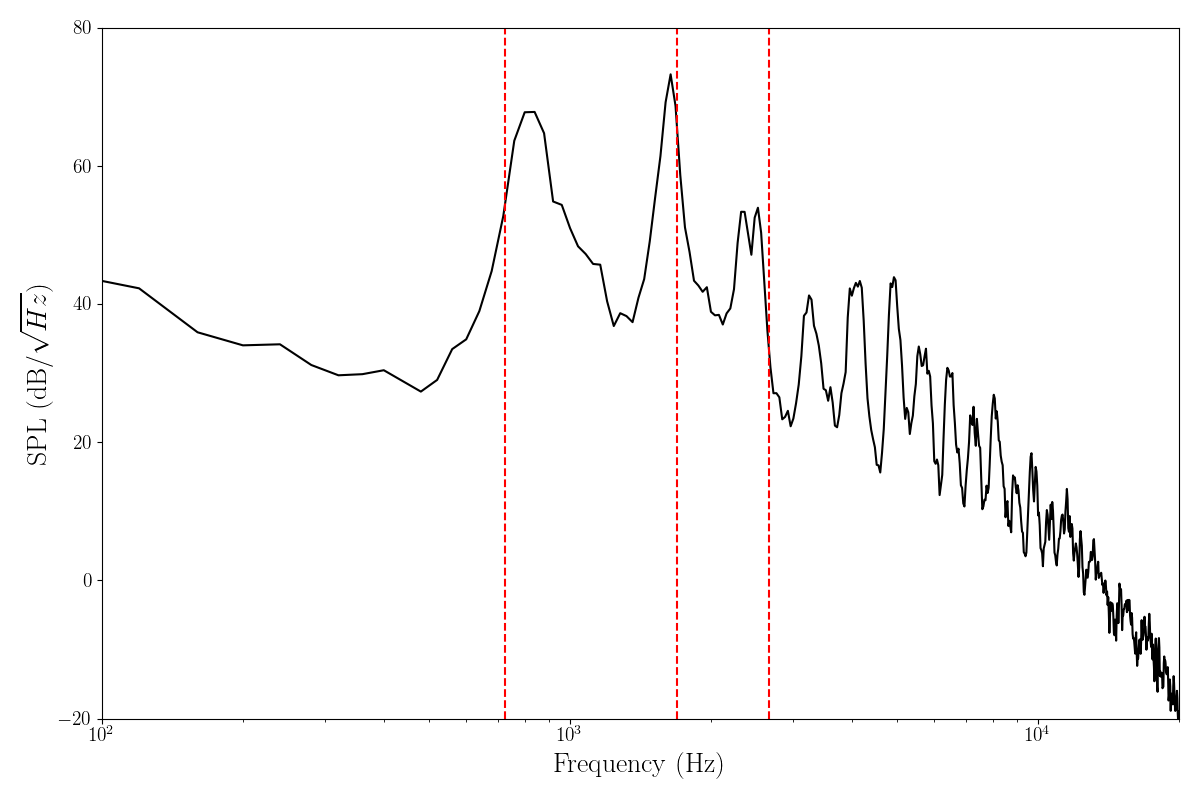
\includegraphics[width=0.99\linewidth]{experiments/2d_cavity/psd_fom_100ms.png}
		\end{minipage}
	\end{figure}

	\footnotetext[12]{\tiny{Tezaur et al., \textit{Tech. report Sandia National Laboratories}, 2017.}}
\end{frame}

\begin{frame}{HPROM performance}
	\begin{figure}
		\begin{minipage}{0.49\linewidth}
			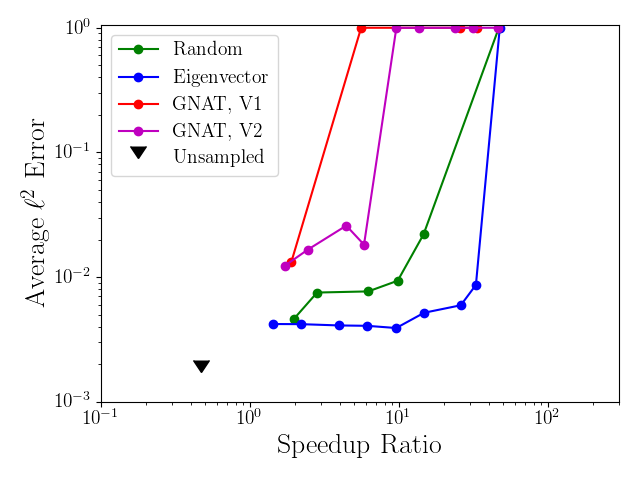
\includegraphics[width=0.99\linewidth]{Images/experiments/2d_cavity/sampled_dt2p5e-6_Average_errorRaw_pareto.png}
		\end{minipage}
		\begin{minipage}{0.4\linewidth}
			\centering
			\animategraphics[autoplay,loop,trim=1em 1em 1em 1em,width=0.75\linewidth,every=40]{10}{Images/experiments/2d_cavity/fom_pressure_zoom/fig_Static_Pressure_zoom_}{108000}{110000}
			
			\centering
			\animategraphics[autoplay,loop,trim=1em 1em 1em 1em,width=0.75\linewidth,every=16]{10}{Images/experiments/2d_cavity/hprom_pressure_zoom/fig_Static_Pressure_zoom_}{43200}{44000}
			\caption*{$\numResModes = 250, \numSamps = 1\%$}
		\end{minipage}
	\end{figure}
	\begin{tcolorbox}[colframe=blue!50!white,halign=center]
		\textbf{Extreme sensitivity} to sampling method	
	\end{tcolorbox}
\end{frame}

\begin{frame}{3D trucated CVRC combustor}
	\begin{itemize}
		\item Truncated single-element gaseous methane-peroxide combustor\footnotemark[13]
		\item Flamelet-progress variable combustion model (GRI-Mech 1.2)
		\item $\sim$18 mil. DOF, 880 cores $\rightarrow$ 30k CPU-h per simulated millisecond
	\end{itemize}
	\begin{figure}
		\begin{minipage}{0.49\linewidth}
				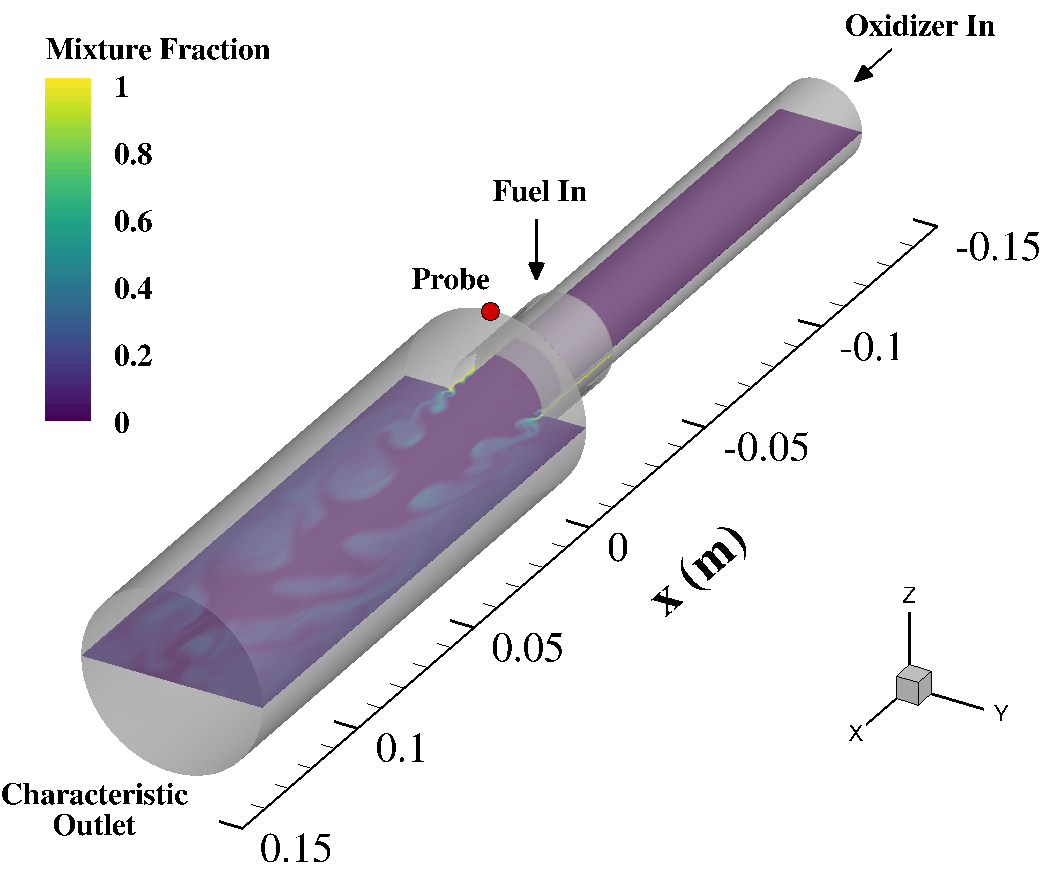
\includegraphics[width=0.95\linewidth]{Images/experiments/cvrc/geom.png}
		\end{minipage}
		\begin{minipage}{0.49\linewidth}
			\animategraphics[autoplay,loop,trim=0.5em 0.5em 0.5em 0.5em,width=0.99\linewidth,every=100]{10}{Images/experiments/cvrc/fom_pressure/fig_z_Static_Pressure_}{50000}{55000}

			\animategraphics[autoplay,loop,trim=0.5em 0.5em 0.5em 0.5em,width=0.99\linewidth,every=100]{10}{Images/experiments/cvrc/fom_temp/fig_z_Temperature_}{50000}{55000}

			\animategraphics[autoplay,loop,trim=0.5em 0.5em 0.5em 0.5em,width=0.99\linewidth,every=100]{10}{Images/experiments/cvrc/fom_z/fig_z_Flamelet_Scalar_Mean_}{50000}{55000}
		\end{minipage}
	\end{figure}

	\footnotetext[13]{\tiny{Harvazinski et al., \textit{Phys. Fluids}, Vol. 27, 2015.}}
\end{frame}

\begin{frame}{Sparse sampling}
	\begin{figure}
		\centering
		\begin{minipage}{0.3\linewidth}
			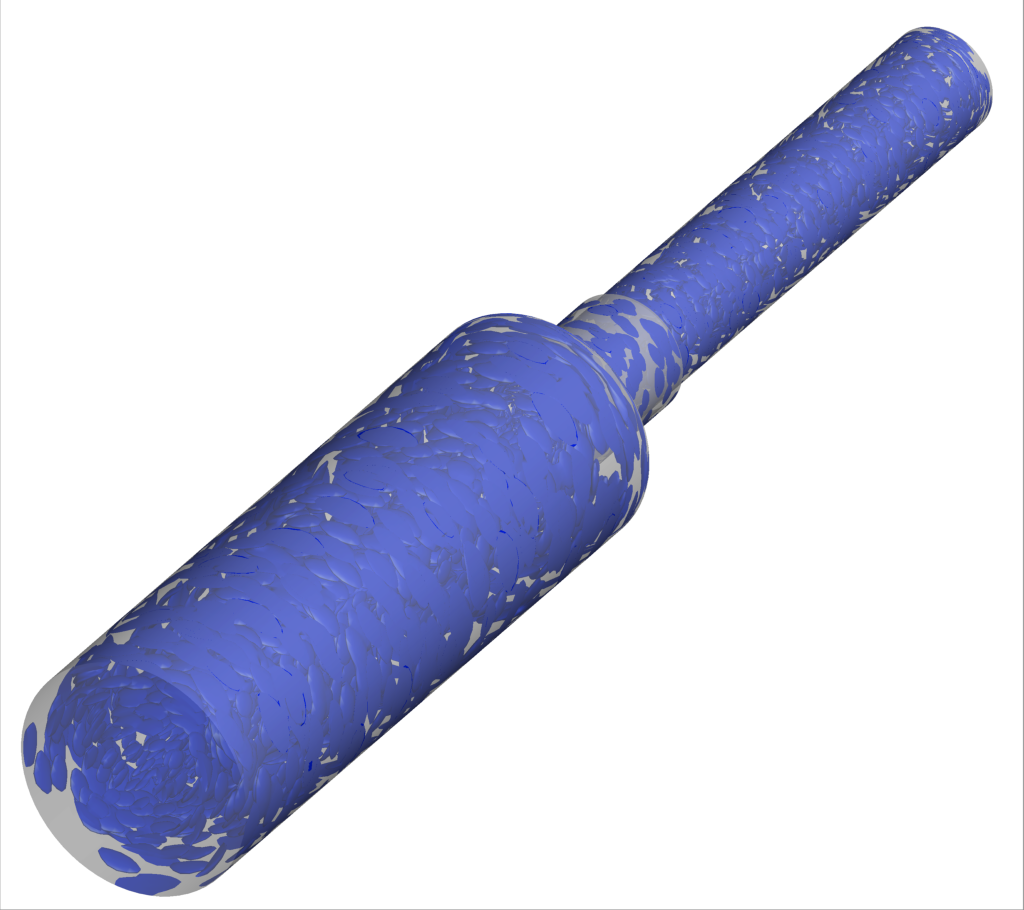
\includegraphics[width=0.99\linewidth,trim={0.5em 0.5em 0.5em 0.5em},clip]{Images/experiments/cvrc/iblank/random_iblank_iso.png}
			\subcaption{Random}
		\end{minipage}
		\begin{minipage}{0.3\linewidth}
			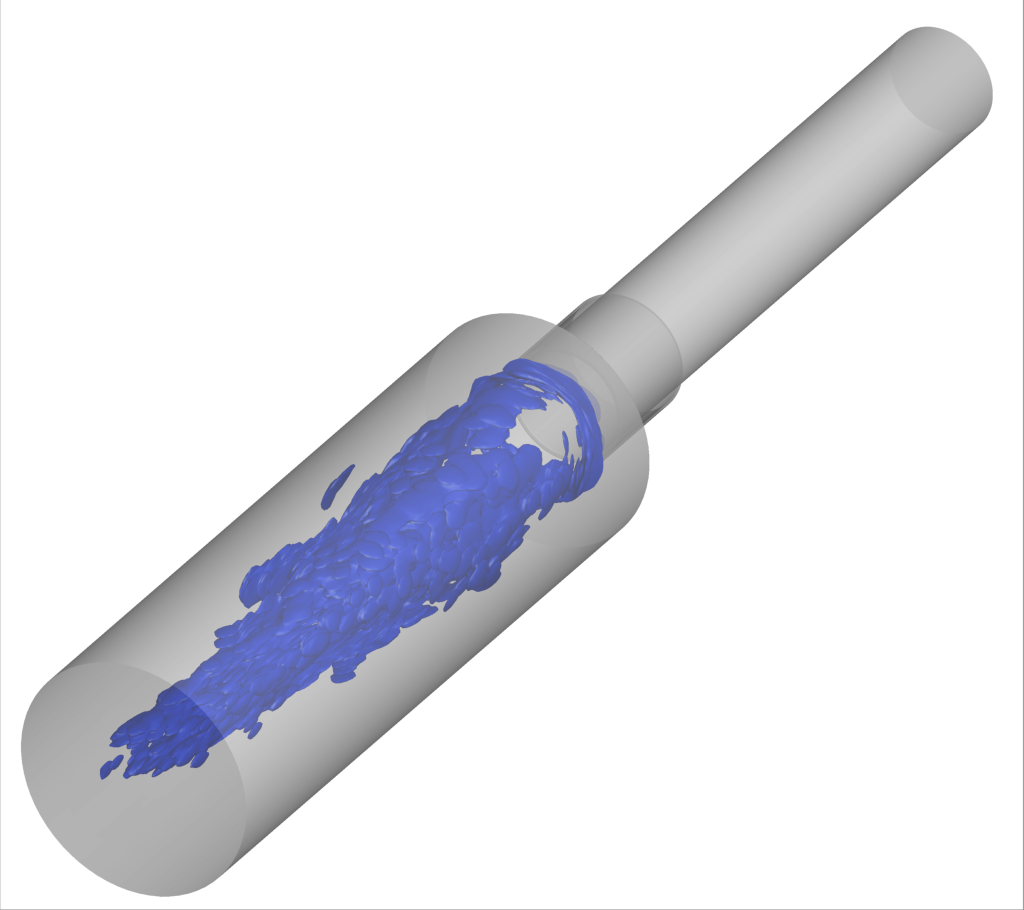
\includegraphics[width=0.99\linewidth,trim={0.5em 0.5em 0.5em 0.5em},clip]{Images/experiments/cvrc/iblank/eigenvec_iblank_iso.png}
			\subcaption{Eigenvector}
		\end{minipage}
	
		\centering
		\begin{minipage}{0.3\linewidth}
			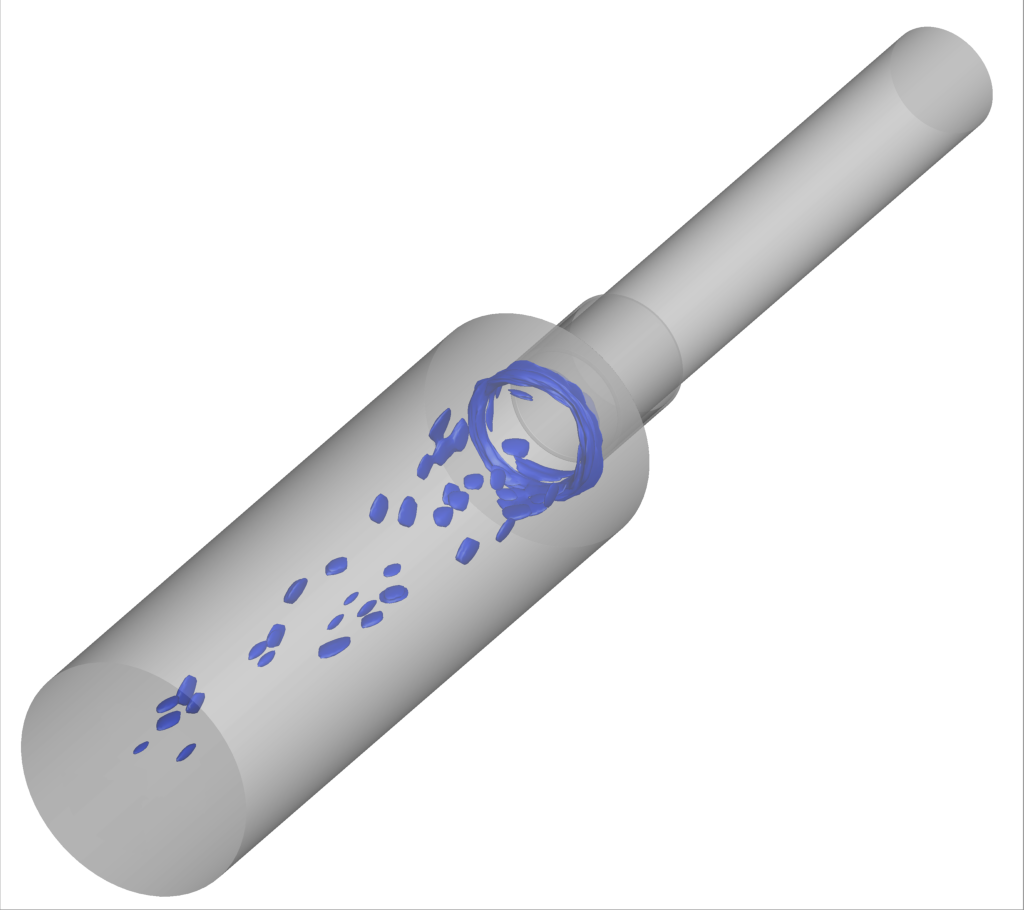
\includegraphics[width=0.99\linewidth,trim={0.5em 0.5em 0.5em 0.5em},clip]{Images/experiments/cvrc/iblank/greedy_carlberg_iblank_iso.png}
			\subcaption{GNAT V1}
		\end{minipage}
		\begin{minipage}{0.3\linewidth}
			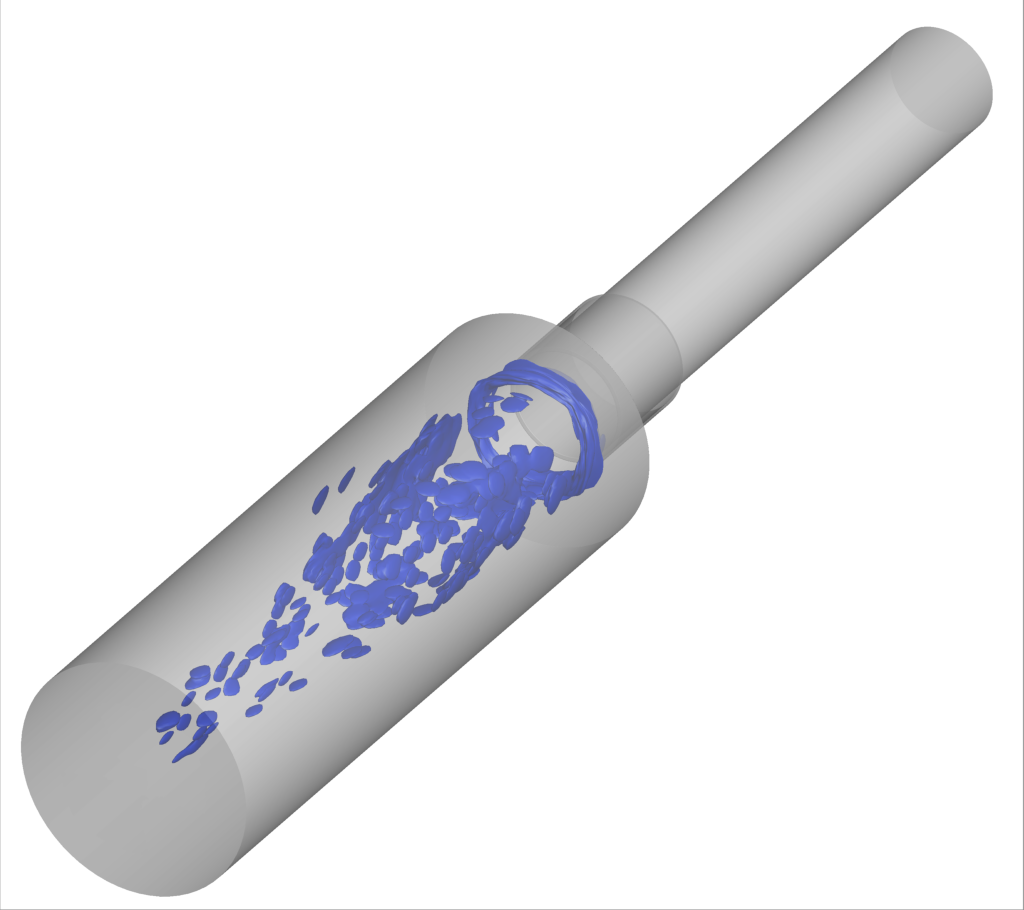
\includegraphics[width=0.99\linewidth,trim={0.5em 0.5em 0.5em 0.5em},clip]{Images/experiments/cvrc/iblank/greedy_ben_iblank_iso.png}
			\subcaption{GNAT V2}
		\end{minipage}
	\end{figure}
\end{frame}

\begin{frame}{Offline cost}
	\begin{itemize}
		\item Sampling cost in terms of FOM iteration cost 
	\end{itemize}
	\begin{figure}
		\begin{minipage}{0.49\linewidth}
			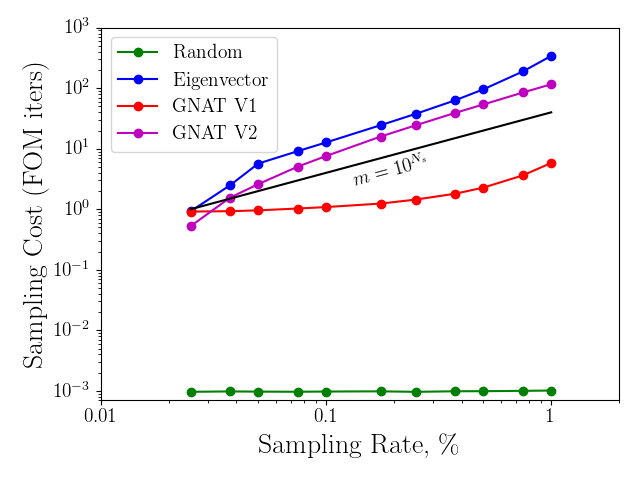
\includegraphics[width=0.99\linewidth]{Images/experiments/cvrc/samp_timing_wrt_samprate.png}
			\caption*{$\numResModes = 300$}
		\end{minipage}
		\begin{minipage}{0.49\linewidth}
			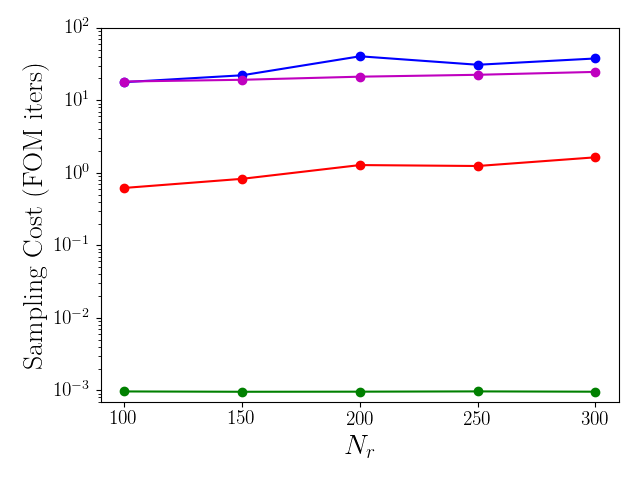
\includegraphics[width=0.99\linewidth]{Images/experiments/cvrc/samp_timing_wrt_modes.png}
			\caption*{$\numSamps = 0.25\% \times \numDOF$}
		\end{minipage}
	\end{figure}
	\begin{tcolorbox}[colframe=blue!50!white,halign=center]
		Random sampling costs \textbf{nothing} \\
		Greedy methods scale \textbf{exponentially} with $\numSamps$
	\end{tcolorbox}
\end{frame}

\begin{frame}{Load balancing (18 mil. DOF)}
	\begin{itemize}
		\item How the mesh is divided between parallel processes
	\end{itemize}
	\begin{figure}
		\begin{minipage}{0.49\linewidth}
			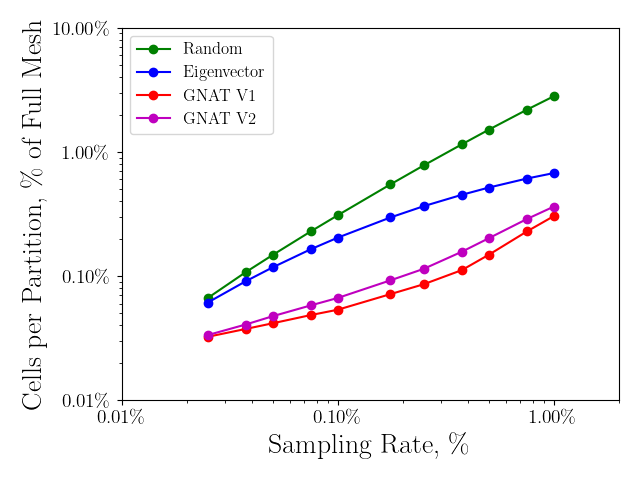
\includegraphics[width=0.99\linewidth]{Images/experiments/cvrc/cvrc_partition_stats.png}
		\end{minipage}
		\begin{minipage}{0.49\linewidth}
			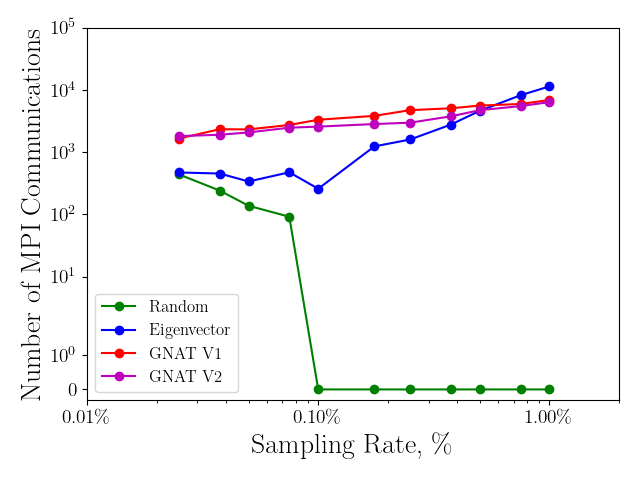
\includegraphics[width=0.99\linewidth]{Images/experiments/cvrc/cvrc_partition_comms.png}
		\end{minipage}
		\caption*{10 partitions, various $\numSamps$.}
	\end{figure}
	\begin{tcolorbox}[colframe=blue!50!white,halign=center]
		Random meshes are \textbf{large}, but \textbf{disjoint} \\
		Greedy meshes are \textbf{small}, but induce \textbf{high MPI overhead}
	\end{tcolorbox}
\end{frame}

\begin{frame}{HPROM performance (18 mil. DOF)}
	\begin{figure}
		\begin{minipage}{0.35\linewidth}
			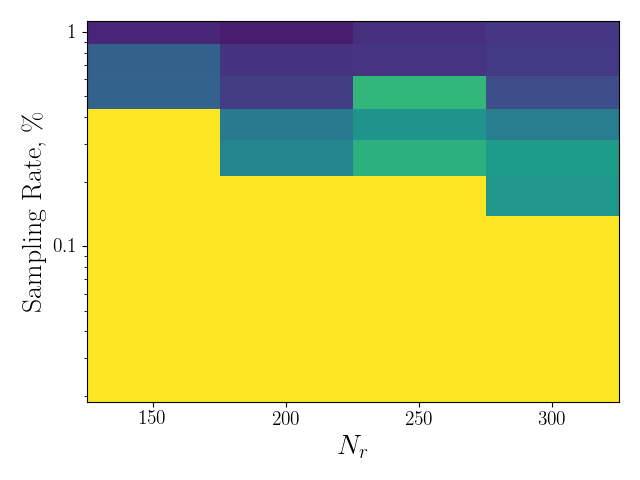
\includegraphics[width=0.99\linewidth]{Images/experiments/cvrc/err_contour_random_dt5e-7.png}
			\subcaption{\scriptsize{Random}}
		\end{minipage}
		\begin{minipage}{0.4\linewidth}
			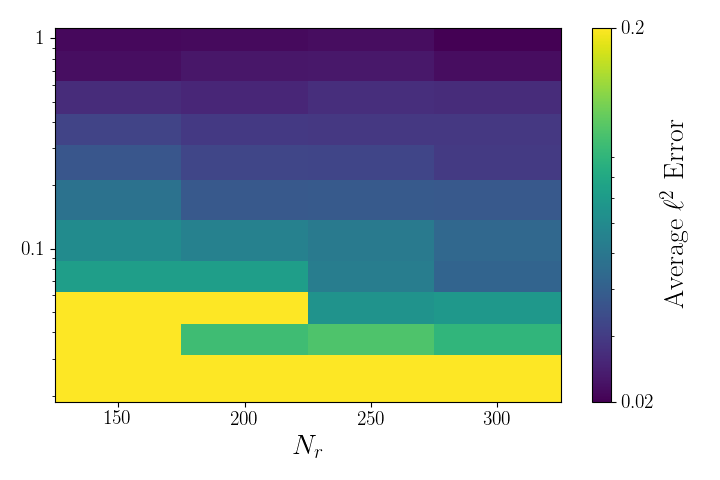
\includegraphics[width=0.99\linewidth]{Images/experiments/cvrc/err_contour_eigenvec_dt5e-7.png}
			\subcaption{\scriptsize{Eigenvector}}
		\end{minipage}
	
		\begin{minipage}{0.35\linewidth}
			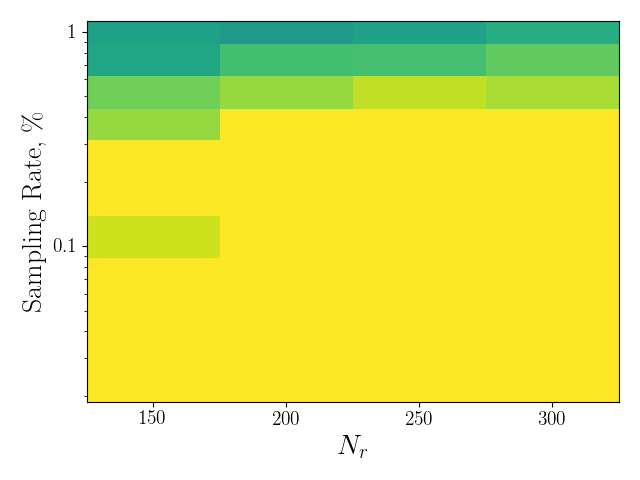
\includegraphics[width=0.99\linewidth]{Images/experiments/cvrc/err_contour_gnat1_dt5e-7.png}
			\subcaption{\scriptsize{GNAT, V1}}
		\end{minipage}
		\begin{minipage}{0.4\linewidth}
			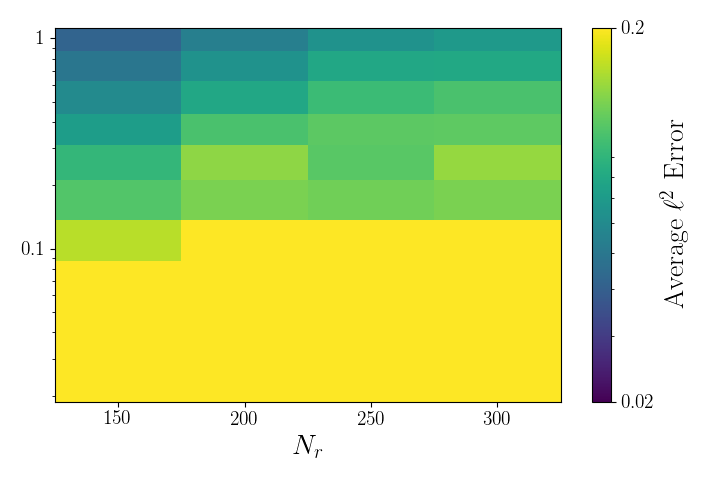
\includegraphics[width=0.99\linewidth]{Images/experiments/cvrc/err_contour_gnat2_dt5e-7.png}
			\subcaption{\scriptsize{GNAT, V2}}
		\end{minipage}
	\end{figure}
\end{frame}

\begin{frame}{HPROM performance (18 mil. DOF)}
	\begin{figure}
		\begin{minipage}{0.49\linewidth}
			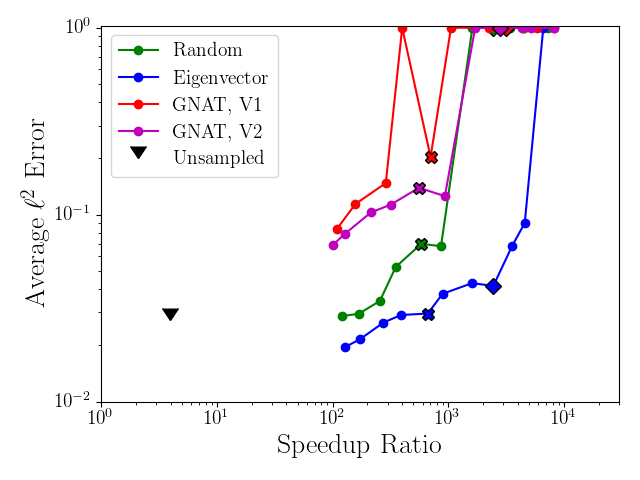
\includegraphics[width=0.99\linewidth]{Images/experiments/cvrc/sampled_dt5e-7_Average_errorRaw_pareto.png}
			\caption*{$\dt = 5 \times \dtFOM$}
		\end{minipage}
		\begin{minipage}{0.49\linewidth}
			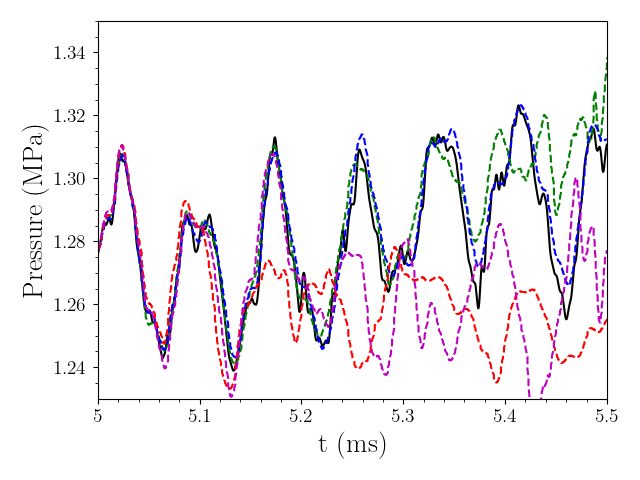
\includegraphics[width=0.99\linewidth]{Images/experiments/cvrc/pressure_probe_deim_dt5e-7_samp0p0025.png}
			\caption*{$\numResModes = 300$, $\numSamps = 0.25\% \times \numDOF$}
		\end{minipage}
	\end{figure}
	\begin{tcolorbox}[colframe=blue!50!white,halign=center]
		\textbf{Eigenvector-based sampling} consistently outperforms \\
		$10^3$-$10^4$ cost savings with \textbf{minimal accuracy loss}
	\end{tcolorbox}
\end{frame}

\begin{frame}{HPROM performance (18 mil. DOF)}
	\begin{minipage}{0.15\linewidth}
		\textbf{FOM}

		\vspace{2.5em}

		\textbf{Random}

		\vspace{2.5em}

		\textbf{Eigenvec}

		\vspace{2.5em}

		\textbf{GNAT V1}

		\vspace{2.5em}

		\textbf{GNAT V2}

	\end{minipage}\hspace{1em}
	\begin{minipage}{0.75\linewidth}
		\begin{figure}
		
			\raisebox{-0.5\height}{\animategraphics[autoplay,loop,trim=0.5em 0.5em 0.5em 0.5em,width=0.81\linewidth,every=50]{10}{Images/experiments/cvrc/fom_temp_comp/fig_z_Temperature_}{52500}{55000}}
			\raisebox{-0.5\height}{\animategraphics[autoplay,loop,trim=0.1em 0.1em 0.1em 0.1em,width=0.14\linewidth,every=50]{10}{Images/experiments/cvrc/fom_temp_comp/fig_x_Temperature_}{52500}{55000}}
	
			\raisebox{-0.5\height}{\animategraphics[autoplay,loop,trim=0.5em 0.5em 0.5em 0.5em,width=0.81\linewidth,every=10]{10}{Images/experiments/cvrc/random_temp/fig_z_Temperature_}{10500}{11000}}
			\raisebox{-0.5\height}{\animategraphics[autoplay,loop,trim=0.1em 0.1em 0.1em 0.1em,width=0.14\linewidth,every=10]{10}{Images/experiments/cvrc/random_temp/fig_x_Temperature_}{10500}{11000}}

			\raisebox{-0.5\height}{\animategraphics[autoplay,loop,trim=0.5em 0.5em 0.5em 0.5em,width=0.81\linewidth,every=10]{10}{Images/experiments/cvrc/eigenvec_temp/fig_z_Temperature_}{10500}{11000}}
			\raisebox{-0.5\height}{\animategraphics[autoplay,loop,trim=0.1em 0.1em 0.1em 0.1em,width=0.14\linewidth,every=10]{10}{Images/experiments/cvrc/eigenvec_temp/fig_x_Temperature_}{10500}{11000}}

			\raisebox{-0.5\height}{\animategraphics[autoplay,loop,trim=0.5em 0.5em 0.5em 0.5em,width=0.81\linewidth,every=10]{10}{Images/experiments/cvrc/gnatv1_temp/fig_z_Temperature_}{10500}{11000}}
			\raisebox{-0.5\height}{\animategraphics[autoplay,loop,trim=0.1em 0.1em 0.1em 0.1em,width=0.14\linewidth,every=10]{10}{Images/experiments/cvrc/gnatv1_temp/fig_x_Temperature_}{10500}{11000}}

			\raisebox{-0.5\height}{\animategraphics[autoplay,loop,trim=0.5em 0.5em 0.5em 0.5em,width=0.81\linewidth,every=10]{10}{Images/experiments/cvrc/gnatv2_temp/fig_z_Temperature_}{10500}{11000}}
			\raisebox{-0.5\height}{\animategraphics[autoplay,loop,trim=0.1em 0.1em 0.1em 0.1em,width=0.14\linewidth,every=10]{10}{Images/experiments/cvrc/gnatv2_temp/fig_x_Temperature_}{10500}{11000}}

		\end{figure}
	\end{minipage}
	
\end{frame}


\begin{frame}{3D nine-element combustor}
	\begin{itemize}
		\item Air Force Center of Excellence ``grand challenge'' case\footnotemark[14]
		\item 12 species, 38 reaction mechanism 
		\item 238 mil. DOF, 2,200 cores $\rightarrow ~\sim$400k CPU-h per 1T mode
	\end{itemize}
	\begin{figure}
		\begin{minipage}{0.45\linewidth}
			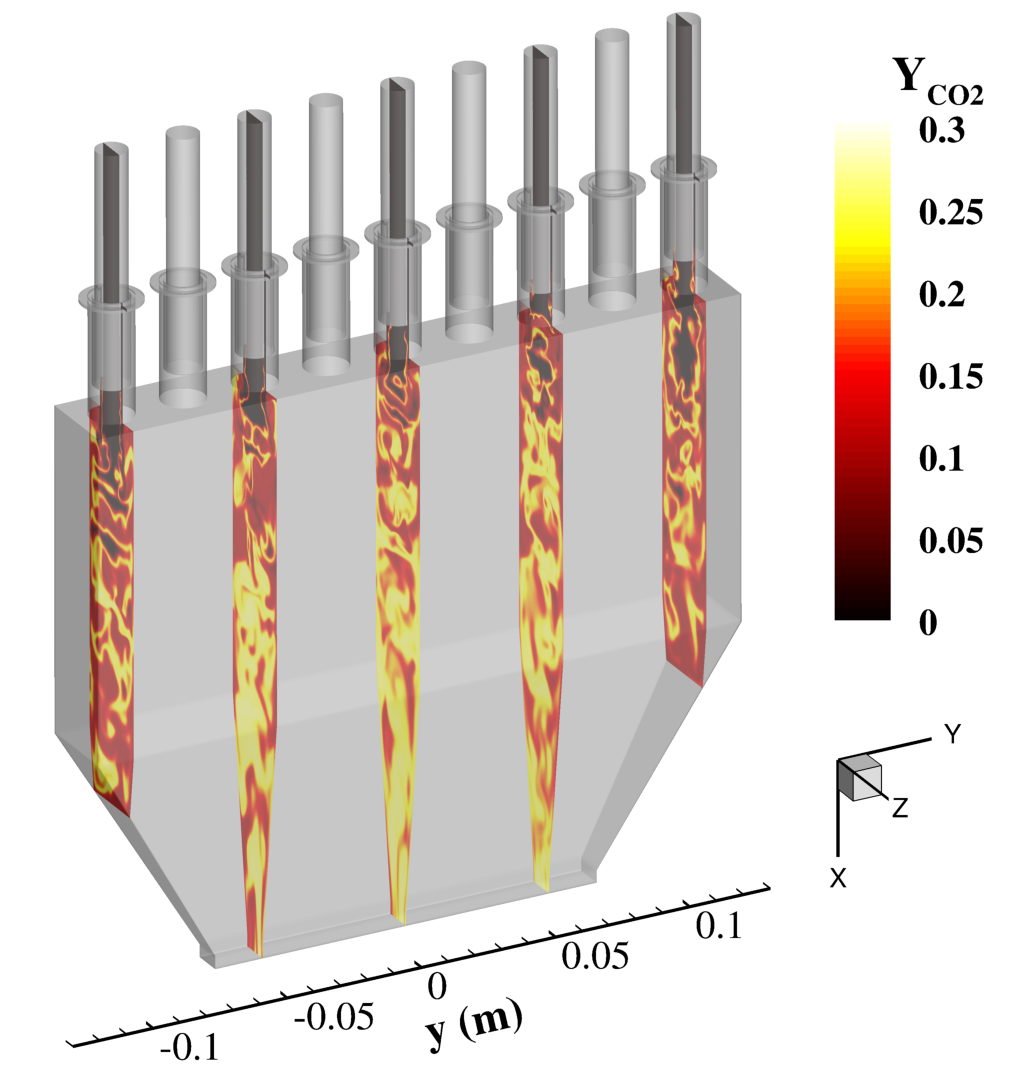
\includegraphics[width=0.99\linewidth]{Images/experiments/9elem/geom_iso.png}
		\end{minipage}
		\begin{minipage}{0.45\linewidth}
			\animategraphics[autoplay,loop,trim=1em 1em 1em 1em,width=0.99\linewidth,every=60]{10}{Images/experiments/9elem/fom_pressure/fig_z_Static_Pressure_}{215000}{218900}
		\end{minipage}
	\end{figure}
	\footnotetext[14]{\tiny{Harvazinski et al., \textit{AIAA Scitech Forum}, 2019}}
\end{frame}

\begin{frame}{Unsampled PROM perfomance}
	\begin{itemize}
		\item Faithful reconstruction with $\numPrimModes \ge 80$
		\item Pressure field lacks some high-frequency content
	\end{itemize}
	\begin{figure}
		\begin{minipage}{0.49\linewidth}
			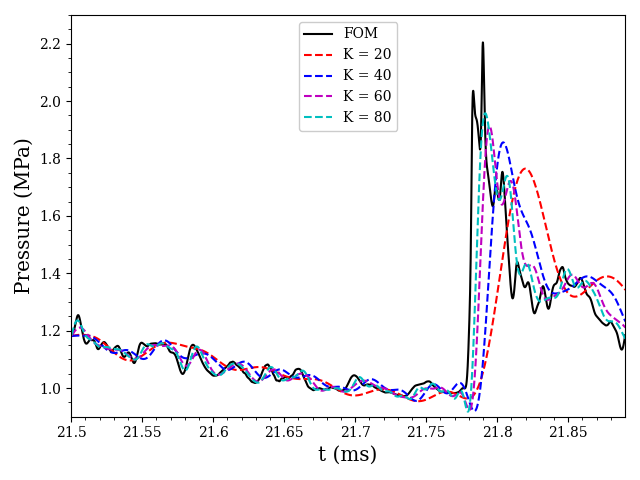
\includegraphics[width=0.99\linewidth]{Images/experiments/9elem/point_3_Static_Pressure.png}
		\end{minipage}
		\begin{minipage}{0.45\linewidth}
			\animategraphics[autoplay,loop,trim=1em 1em 1em 1em,width=0.99\linewidth,every=2]{6}{Images/experiments/9elem/rom_pressure/fig_z_Static_Pressure_}{4302}{4380}
		\end{minipage}
	\end{figure}
\end{frame}

\begin{frame}{HPROM takeaways}
	\begin{itemize}
		\item MP-LSVT exhibits excellent stability and accuracy
		\item Offline cost of greedy methods can be significant
		\item Performance is extremely sensitive to sampling algorithm
		\begin{itemize}
			\item Eigenvector-based sampling is clear victor
			\item Traditional GNAT often worse than random sampling
		\end{itemize}
		\item Over three orders of magnitude cost savings
		\item Faithful modeling of complex combustion phenomena
	\end{itemize}
\end{frame}

\section*{Adaptive PROMs}

\begin{frame}{Predictive PROMs}
	\begin{itemize}
		\item Out-of-training predictions
		\begin{itemize}
			\item Future-state
			\item Parametric variations (BC's, reaction, etc.)
			\item Geometric variations
		\end{itemize}
		\item Static trial space cannot represent unseen data
	\end{itemize}
	\begin{figure}
		\begin{minipage}{0.49\linewidth}
			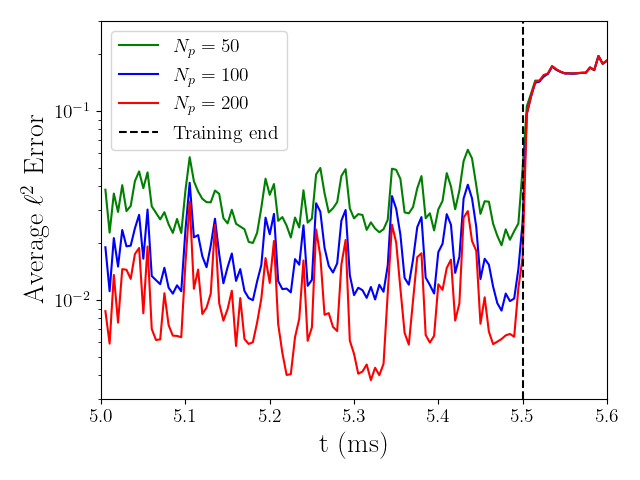
\includegraphics[width=0.9\linewidth]{Images/experiments/cvrc/proj_err_time.png}
		\end{minipage}	
		\begin{minipage}{0.49\linewidth}
			\animategraphics[autoplay,loop,trim={0.5em 0.5em 0.5em 0.5em},clip,width=0.99\linewidth,every=40]{10}{Images/experiments/cvrc/fom_temp_adapt/fig_z_Temperature_}{54000}{56000}	
			
			\animategraphics[autoplay,loop,trim={0.5em 0.5em 0.5em 0.5em},clip,width=0.99\linewidth,every=40]{10}{Images/experiments/cvrc/proj_temp/fig_z_Temperature_}{54000}{56000}	
		\end{minipage}
	\end{figure}
	\begin{tcolorbox}[colframe=blue!50!white,halign=center]
		True predictivity requires \textbf{adaptation}
	\end{tcolorbox}
\end{frame}

\begin{frame}{Basis and sampling adaptation}
	\begin{itemize}
		\item Periodic queries of full-order operator at interval $\updateFreq$
		\item AADEIM\footnotemark[15] sampling update criterion
		\begin{equation*}
			\argmax{} \primVec - \primTrial \left[\sampMat \primTrial\right]^+ \sampMat \primVecRom
		\end{equation*}
		\item One-step basis adaptation\footnotemark[16]
		\begin{equation*}
			\primVec^{\timeIdx} = \primVecCent + \primScale \left[\primTrial^{\timeIdx} + \left[\primTrialUpdate\right]^{\timeIdx} \right] \primVecCoef^{\timeIdx},
		\end{equation*}
		\begin{equation*}
			\sampMat^{\timeIdx} [\primTrialUpdate]^{\timeIdx+1} = \sampMat^{\timeIdx} [\primTrialUpdate]^{\timeIdx} + \frac{\sampMat^{\timeIdx} \left[\primScaleInv\left[\primVec^{\timeIdx} - \primVecCent\right] - \primTrial^{\timeIdx} \primVecCoef^{\timeIdx}\right]\left[\primVecCoef^{\timeIdx}\right]^\top}{\left\Vert \primVecCoef^{\timeIdx} \right\Vert^2_2}
		\end{equation*}
	\end{itemize}

	\footnotetext[15]{\tiny{Peherstorfer and Willcox, \textit{SIAM J Sci. Comp.}, Vol. 37, 2015.}}
	\footnotetext[16]{\tiny{Huang and Duraisamy, \textit{arXiv:2301.09006}, 2023}}
\end{frame}

\begin{frame}{CVRC future-state predictions}
	\begin{itemize}
		\item Train only on first 0.005 ms, predict for 0.5 ms
		\item Small trial basis, $\numPrimModes \le 10$ 
	\end{itemize}
	\begin{figure}
			% probe showing training bound
			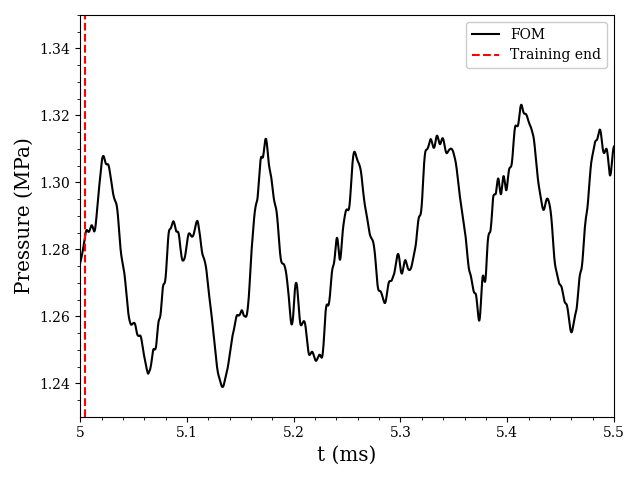
\includegraphics[width=0.5\linewidth]{Images/experiments/cvrc/press_fom_train_bound.png}
	\end{figure}
	\begin{tcolorbox}[colframe=blue!50!white,halign=center]
		Adaptive PROM incurs \textbf{miniscule offline cost}
	\end{tcolorbox}
\end{frame}

\begin{frame}{Adaptive HPROM performance}
	\begin{itemize}
		\item Increasing $\updateFreq$ decreases cost, causes solution to ``drag''
	\end{itemize}
	\begin{figure}
		\begin{minipage}{0.49\linewidth}
			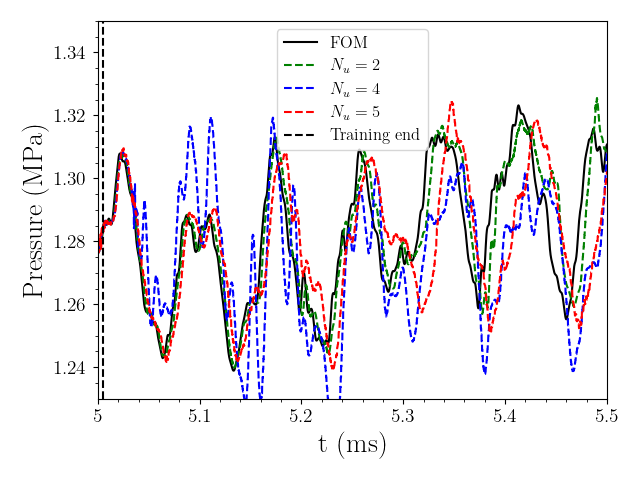
\includegraphics[width=0.99\linewidth]{Images/experiments/cvrc/pressure_probe_wrt_iter.png}
		\end{minipage}
		\begin{minipage}{0.49\linewidth}
			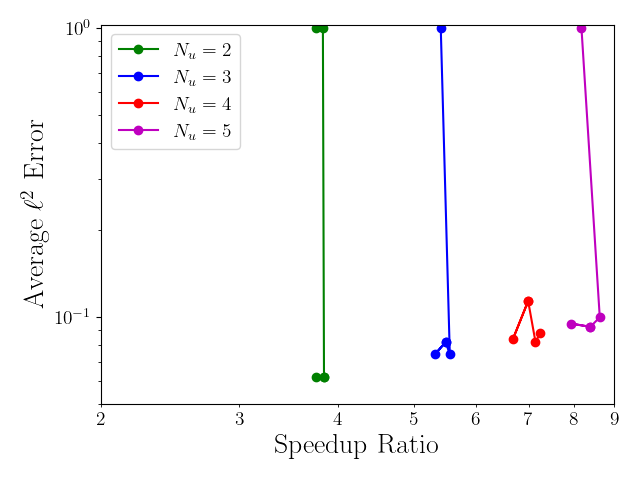
\includegraphics[width=0.99\linewidth]{Images/experiments/cvrc/pareto_wrt_iters_Average_errorRaw_pareto.png}
		\end{minipage}
	\end{figure}

\end{frame}

\begin{frame}{Adaptive HPROM performance}
	\begin{minipage}{0.15\linewidth}
		\textbf{FOM}

		\vspace{2.5em}

		$\mathbf{\updateFreq = 2}$

		\vspace{2.5em}

		$\mathbf{\updateFreq = 4}$

		\vspace{2.5em}

		$\mathbf{\updateFreq = 5}$

	\end{minipage}\hspace{2em}
	\begin{minipage}{0.75\linewidth}
		\begin{figure}
		
			\raisebox{-0.5\height}{\animategraphics[autoplay,loop,trim=0.5em 0.5em 0.5em 0.5em,width=0.81\linewidth,every=100]{10}{Images/experiments/cvrc/fom_temp_adapt_rom/fig_z_Temperature_}{50100}{55000}}
			\raisebox{-0.5\height}{\animategraphics[autoplay,loop,trim=0.1em 0.1em 0.1em 0.1em,width=0.14\linewidth,every=100]{10}{Images/experiments/cvrc/fom_temp_adapt_rom/fig_x_Temperature_}{50100}{55000}}

			\raisebox{-0.5\height}{\animategraphics[autoplay,loop,trim=0.5em 0.5em 0.5em 0.5em,width=0.81\linewidth,every=2]{10}{Images/experiments/cvrc/adapt_freq2/fig_z_Temperature_}{1002}{1100}}
			\raisebox{-0.5\height}{\animategraphics[autoplay,loop,trim=0.1em 0.1em 0.1em 0.1em,width=0.14\linewidth,every=2]{10}{Images/experiments/cvrc/adapt_freq2/fig_x_Temperature_}{1002}{1100}}

			\raisebox{-0.5\height}{\animategraphics[autoplay,loop,trim=0.5em 0.5em 0.5em 0.5em,width=0.81\linewidth,every=2]{10}{Images/experiments/cvrc/adapt_freq4/fig_z_Temperature_}{1002}{1100}}
			\raisebox{-0.5\height}{\animategraphics[autoplay,loop,trim=0.1em 0.1em 0.1em 0.1em,width=0.14\linewidth,every=2]{10}{Images/experiments/cvrc/adapt_freq4/fig_x_Temperature_}{1002}{1100}}

			\raisebox{-0.5\height}{\animategraphics[autoplay,loop,trim=0.5em 0.5em 0.5em 0.5em,width=0.81\linewidth,every=2]{10}{Images/experiments/cvrc/adapt_freq5/fig_z_Temperature_}{1002}{1100}}
			\raisebox{-0.5\height}{\animategraphics[autoplay,loop,trim=0.1em 0.1em 0.1em 0.1em,width=0.14\linewidth,every=2]{10}{Images/experiments/cvrc/adapt_freq5/fig_x_Temperature_}{1002}{1100}}

		\end{figure}
	\end{minipage}
\end{frame}

\begin{frame}{Adaptive PROM takeaways}
	\begin{itemize}
		\item Reasonable predictions where static basis fails outright
		\item Increasing update threshold $\updateFreq$
		\begin{itemize}
			\item Deteriorates point-wise measurements
			\item Retains qualitative flow field behavior
		\end{itemize}
		\item Absolute speedup threshold dictated by $\updateFreq$
		\item Adaptive PROM is \textbf{not} independent of $\numDOF$
	\end{itemize}

	\begin{equation*}
		\lambda \le \updateFreq \frac{k_{\text{ROM}}}{k_{\text{FOM}}} 
	\end{equation*}
\end{frame}

\section*{Best Practices}

\begin{frame}{Best practices}
	\begin{itemize}
		\item Literature often glosses over small, critical details
		\item Feature scaling
		\begin{equation*}
			\primVecRom = \primVecCent + \primScale \primTrial \primVecCoef
		\end{equation*}
		\item Residual non-dimensionalization
		\begin{equation*}
			\delta \primVecCoef^{\newtonIdx, \timeIdx} = \argmin{\dummyVec \in \mathbb{R}^{\numPrimModes}} \norm{\resScaleInv \left(\pde{\resFuncIter{\timeIdx}{\dummyVec}}{\dummyVec} \dummyVec + \resFuncIter{\timeIdx}{\dummyVec}\right)}_2^2
		\end{equation*}
		\item Local limiters
		\begin{equation*}
			\temperature = min\left(max\left(\temperature, \; \temperature_{min}\right), \; \temperature_{max}\right)
		\end{equation*}
		\item Sampling algorithm
	\end{itemize}
\end{frame}

\begin{frame}{Best practices: feature scaling}
	\begin{itemize}
		\item Data preparation is crucial for accurate trial space
		\item Centering: initial condition, mean field
		\item Scaling: $\ell^2$-norm, min-max
	\end{itemize}
	\begin{figure}
		\only<1>{
			\begin{minipage}{0.32\linewidth}
				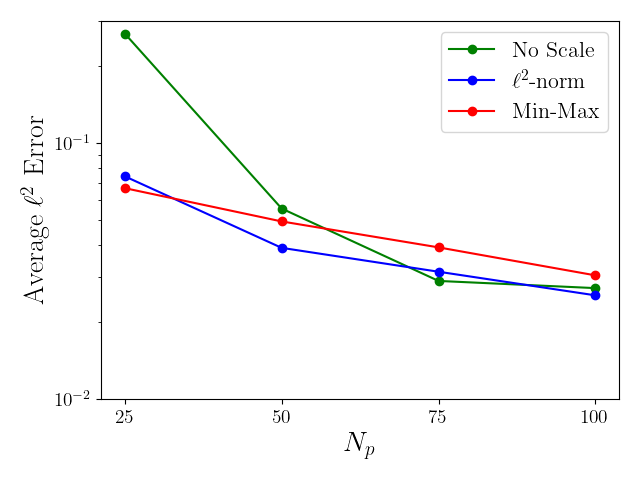
\includegraphics[width=0.99\linewidth]{Images/experiments/cvrc/best_pract/errVsModes_centScale_centNone_Average_errorRaw.png}
				\caption*{No centering}
			\end{minipage}
			\begin{minipage}{0.32\linewidth}
				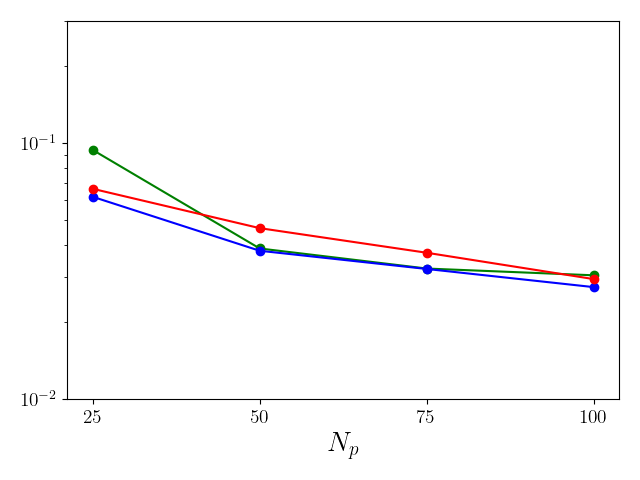
\includegraphics[width=0.99\linewidth]{Images/experiments/cvrc/best_pract/errVsModes_centScale_centIC_Average_errorRaw.png}
				\caption*{IC centering}
			\end{minipage}
			\begin{minipage}{0.32\linewidth}
				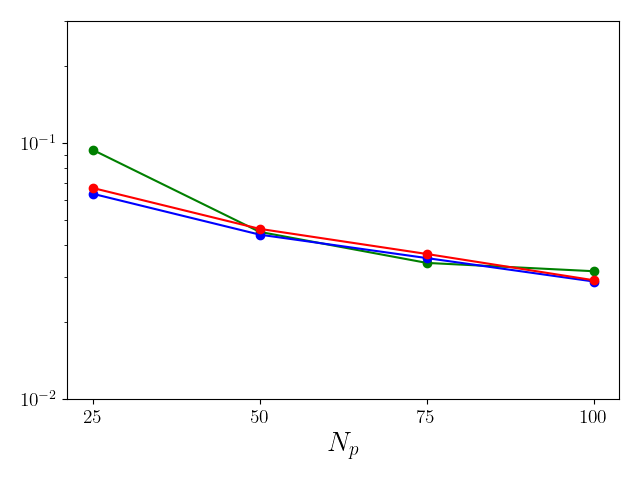
\includegraphics[width=0.99\linewidth]{Images/experiments/cvrc/best_pract/errVsModes_centScale_centMean_Average_errorRaw.png}
				\caption*{Mean centering}
			\end{minipage}
		}
		\only<2>{
			\begin{minipage}{0.32\linewidth}
				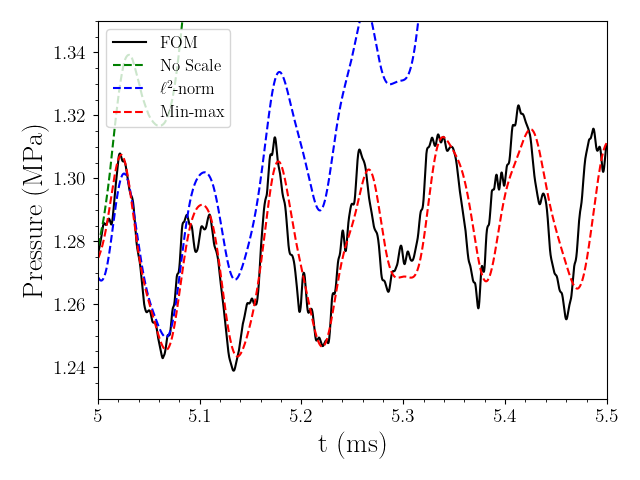
\includegraphics[width=0.99\linewidth]{Images/experiments/cvrc/best_pract/pressure_probe_centScale_centNone.png}
				\caption*{No centering}
			\end{minipage}
			\begin{minipage}{0.32\linewidth}
				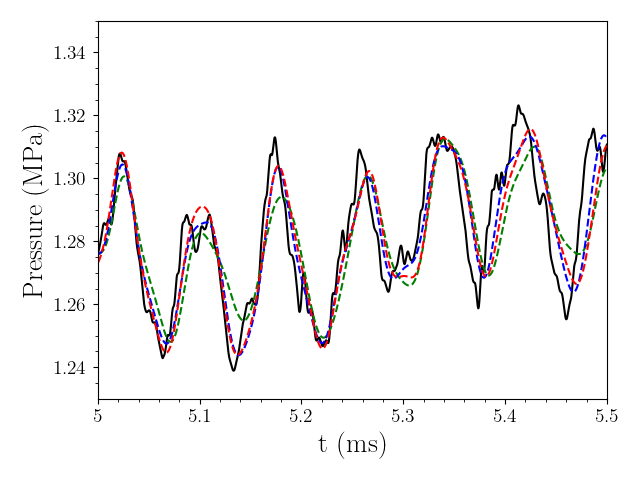
\includegraphics[width=0.99\linewidth]{Images/experiments/cvrc/best_pract/pressure_probe_centScale_centIC.png}
				\caption*{IC centering}
			\end{minipage}
			\begin{minipage}{0.32\linewidth}
				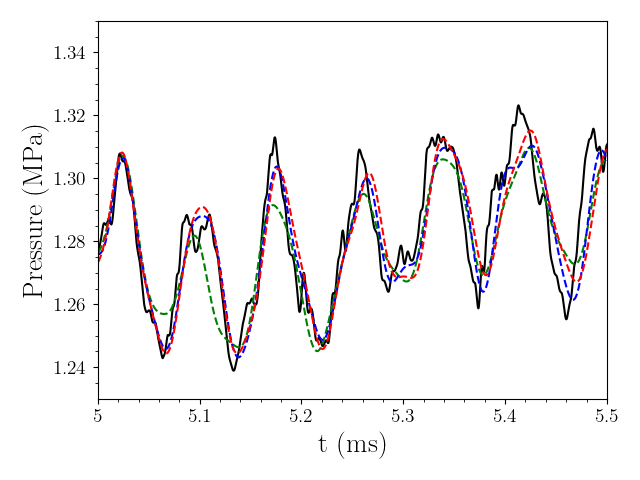
\includegraphics[width=0.99\linewidth]{Images/experiments/cvrc/best_pract/pressure_probe_centScale_centMean.png}
				\caption*{Mean centering}
			\end{minipage}
		}
	\end{figure}
	\begin{tcolorbox}[colframe=blue!50!white,halign=center]
		Centering/scaling are \textbf{required}, \\
		exact method not as important
	\end{tcolorbox}
\end{frame}

\begin{frame}{Best practices: residual non-dimensionalization}
	\begin{itemize}
		\item Failing to non-dimensionalize ROMs leads to poor conditioning
		\item Scaling dataset: $\consVec$, $\rhsFunc{\cdot}$
		\item Scaling method: $\ell^2$-norm, min-max
	\end{itemize}
	\begin{figure}
		\centering
		% \only<1>{
			\begin{minipage}{0.4\linewidth}
				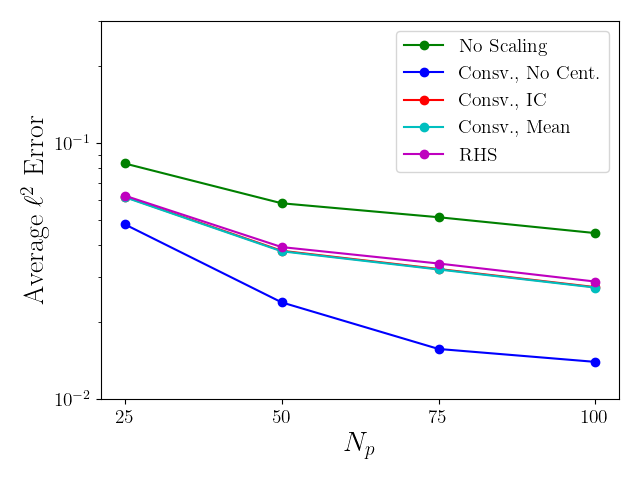
\includegraphics[width=0.99\linewidth]{Images/experiments/cvrc/best_pract/errVsModes_norm_l2_Average_errorRaw.png}
				\caption*{$\ell^2$-norm scaling}
			\end{minipage}
			\begin{minipage}{0.4\linewidth}
				\includegraphics[width=0.99\linewidth]{Images/experiments/cvrc/best_pract/errVsModes_norm_minmax_Average_errorRaw.png}
				\caption*{Min-max scaling}
			\end{minipage}
		% }
		% \only<2>{
		% 	\begin{minipage}{0.4\linewidth}
		% 		\includegraphics[width=0.99\linewidth]{Images/experiments/cvrc/best_pract/pressure_probe_scale_l2.png}
		% 		\caption*{$\ell^2$-norm scaling}
		% 	\end{minipage}
		% 	\begin{minipage}{0.4\linewidth}
		% 		\includegraphics[width=0.99\linewidth]{Images/experiments/cvrc/best_pract/pressure_probe_scale_minmax.png}
		% 		\caption*{Min-max scaling}
		% 	\end{minipage}
		% }
	\end{figure}
	\begin{tcolorbox}[colframe=blue!50!white,halign=center]
		Residual scaling \textbf{halves} time-average error %\\
		% \textbf{Conservative variable} scaling minimizes solution ``drag''
	\end{tcolorbox}
\end{frame}

\begin{frame}{Best practices: local limiters}
	\begin{itemize}
		\item ``Ringing'' from linear trial basis can lead to large over/undershoots
		\item Bound below by fuel temperature, above by AFT 
	\end{itemize}
	\begin{figure}
		\centering
		\begin{minipage}{0.6\linewidth}
			\includegraphics[width=0.99\linewidth]{Images/experiments/cvrc/press_probe_limiters.png}
		\end{minipage}
	\end{figure}
	\begin{tcolorbox}[colframe=blue!50!white,halign=center]
		System-specific limiters are a \textbf{simple hot-fix}
	\end{tcolorbox}
\end{frame}

\begin{frame}{Best practices: sparse sampling}
	\begin{itemize}
		\item Traditional sampling methods did not suffice
	\end{itemize}
	\begin{figure}
		\begin{minipage}{0.49\linewidth}
			\includegraphics[width=0.99\linewidth]{Images/experiments/2d_cavity/sampled_dt2p5e-6_Average_errorRaw_pareto.png}
			\caption*{Cavity}
		\end{minipage}
		\begin{minipage}{0.49\linewidth}
			\includegraphics[width=0.99\linewidth]{Images/experiments/cvrc/sampled_dt5e-7_Average_errorRaw_pareto.png}
			\caption*{CVRC}
		\end{minipage}
	\end{figure}
	\begin{tcolorbox}[colframe=blue!50!white,halign=center]
		Eigenvector-based sampling promotes \textbf{fast} and \textbf{accurate} solutions \\
		Random sampling offers \textbf{inexpensive} early experimentation
	\end{tcolorbox}
\end{frame}

\section*{Conclusions}

\begin{frame}{Contributions}
    \begin{enumerate}
		\item PERFORM, open-source Python package for rapid prototyping novel ROM methods, challenging benchmarks
		\item Scalable PROM solver in high-performance combustion CFD code
        \item State-of-the-art PROMs for multi-scale, multi-physics flow systems
        \item Analysis of cost and performance of sparse sampling methods
        \item First study of PROMs for 3D multi-injector rocket combustor, containing $>$ 250 million DOFs
        \item Truly predictive PROMs for single-element rocket combutor
        \item Best practices for PROMs of multi-scale systems
    \end{enumerate}
\end{frame}


\begin{frame}{Publications and presentations}
	\begin{itemize}
		\item Under review
		\vspace{0.5em}
		\begin{itemize}
			\item \tiny \textbf{Wentland, C.R.}, Huang, C., and Duraisamy, K., ``Scalable Projection-based Reduced-order Models for Large Multi-scale Fluid Systems,'' AIAA Journal, submitted for review.
		\end{itemize}
		\item \normalsize Journal articles
		\vspace{0.5em}
		\begin{itemize}
			\item \tiny Arnold-Medabalimi, N., \textbf{Wentland, C. R.}, Huang, C., and Duraisamy, K., ``PLATFORM: Parallel Linear Algebra Tool FOr
			Reduced Modeling,'' \textit{SoftwareX}, Vol. 21, 2023.
			\item \textbf{Wentland, C.R.} and Duraisamy, K., ``PERFORM: A Python package for developing reduced-order models for reacting fluid flows,'' \textit{J. Open Source Softw.}, 2022.
			\item Huang, C., \textbf{Wentland, C.R.}, Duraisamy, K., and Merkle, C., ``Model reduction for multi-scale transport problems using model-form preserving least-squares projections with variable transformation,'' \textit{J. Comp. Phys.}, 2021, Vol. 448, 2021.
        	\item Parish, E.J., \textbf{Wentland, C.R.}, Duraisamy, K., ``The Adjoint Petrov--Galerkin method for non-linear model reduction,'' \textit{Comput. Method Appl. M.}, Vol. 365, 2020.
		\end{itemize}
		\item \normalsize Conference proceedings
		\vspace{0.5em}
		\begin{itemize}
			\item \tiny \textbf{Wentland, C.R.}, Huang, C., and Duraisamy, K., ``Investigation of Sampling Strategies for Reduced-Order Models of Rocket Combustors,'' \textit{AIAA Scitech Forum}, 2021.
			\item \textbf{Wentland, C.R.}, Huang, C., and Duraisamy, K., ``Closure of Reacting Flow Reduced-Order Models via the Adjoint Petrov-Galerkin Method,'' \textit{AIAA Aviation Forum}, 2019.
		\end{itemize}
		\item \normalsize Conference presentations
		\vspace{0.5em}
		\begin{itemize}
			\item \tiny \textbf{Wentland, C.R.} and Duraisamy, K., ``Intrusive and Non-intrusive Non-linear Reduced-order Models for Reacting Flows,'' \textit{2021 Annual Meeting of the APS Division of Fluid Dynamics}, Phoenix, AZ, USA.
			\item \textbf{Wentland, C.R.}, Nair, A.S., and Duraisamy, K., ``Nonlinear Manifold Reduced-Order Models for Complex Fluid Flow Systems,'' \textit{2021 SIAM Conference on Computational Science and Engineering}, virtual.
			\item \tiny \textbf{Wentland, C.R.}, Parish, E.J., and Duraisamy, K., ``Closure of Reduced-Order Models Using Statistical Mechanics Approaches,'' \textit{2018 World Congress on Computational Mechanics}, New York, NY, USA.
		\end{itemize}
	\end{itemize}
\end{frame}

\begin{frame}{Financial and compute support}
	\begin{itemize}
	    \item Financial support from the US Air Force through the Center of Excellence Grant FA9550-17-1-0195
	    \item Compute support from the US Department of Defense High Performance Computing Modernization Program
		\item Compute support of ConFlux and Lighthouse systems from the University of Michigan Advanced Research Computing division
	\end{itemize}
	\begin{minipage}{0.15\linewidth}
		\vspace{0.5em}
		\begin{figure}
			\includegraphics[width=0.99\linewidth]{back_matter/afrlLogo.png}
		\end{figure}
	\end{minipage}
	\begin{minipage}{0.34\linewidth}
		\begin{figure}
			\includegraphics[width=0.99\linewidth,trim={2cm 3cm 0em 3cm},clip]{back_matter/afosr.jpg}
		\end{figure}
	\end{minipage}
	\begin{minipage}{0.23\linewidth}
		\begin{figure}
			\includegraphics[width=0.99\linewidth]{back_matter/hpcmp.png}
		\end{figure}
	\end{minipage}
	\begin{minipage}{0.23\linewidth}
		\begin{figure}
			\includegraphics[width=0.99\linewidth,trim={0em 3cm 0em 3cm},clip]{back_matter/arc.png}
		\end{figure}
	\end{minipage}
\end{frame}

\begin{frame}[noframenumbering]{Acknowledgements}
	\begin{figure}
		\begin{minipage}{0.49\linewidth}
			\centering
			\includegraphics[width=0.85\linewidth]{Images/ack/PXL_20210904_023138814.jpg}
			\vspace{-1em}
			\includegraphics[angle=270,width=0.85\linewidth,trim={100em 0em 100em 0em},clip]{Images/ack/IMG_3559.jpg}
			
		\end{minipage}
		\begin{minipage}{0.49\linewidth}
			\centering
			\includegraphics[width=0.49\linewidth]{Images/ack/pic_group.jpg}
			\includegraphics[width=0.49\linewidth]{Images/ack/image_cedar.png}

			\centering
			\includegraphics[width=0.85\linewidth]{Images/ack/PXL_20211127_170237667.MP.jpg}
		\end{minipage}
	\end{figure}
\end{frame}

\begin{frame}[noframenumbering]{Acknowledgements}
	\begin{figure}
		\begin{minipage}{0.49\linewidth}
			\centering
			\includegraphics[width=0.8\linewidth,trim={0em 20em 0em 70em},clip]{Images/ack/IMG_2073.JPG}

			\includegraphics[width=0.8\linewidth,trim={0em 0em 0em 20em},clip]{Images/ack/IMG_4210.jpg}

			\includegraphics[width=0.8\linewidth,trim={0em 0em 0em 30em},clip]{Images/ack/IMG_6974.jpg}
		\end{minipage}
		\begin{minipage}{0.49\linewidth}
			\centering
			\includegraphics[width=0.8\linewidth,trim={0em 20em 0em 20em},clip]{Images/ack/IMG_0564.JPG}

			\includegraphics[width=0.8\linewidth,trim={0em 0em 0em 10em},clip]{Images/ack/IMG_7124.jpg}

			\includegraphics[width=0.8\linewidth,trim={0em 30em 0em 0em},clip]{Images/ack/IMG_5132.jpg}
		\end{minipage}
	\end{figure}
\end{frame}

\begin{frame}[noframenumbering]
	\Large
	\centering
	Backup Slides
	\normalsize
\end{frame}

\begin{frame}[noframenumbering]{Acoustically-forced model premixed flame details}
	\begin{itemize}
		\item Fictitious ``reactant'' converts to ``product''
		\item 1,024 cells $\rightarrow$ 4,096 DOF
		\item Sinusoidal forcing about far-field pressure
		\item $\dt = 25$ ns, 2,001 snapshots per FOM simulation
	\end{itemize}
	\begin{minipage}{0.58\linewidth}
		\includegraphics[width=0.99\linewidth]{Images/experiments/transientFlame/fom_press_snaps.png}
	\end{minipage}
	\begin{minipage}{0.39\linewidth}
		\scriptsize
		\begin{table}
			\centering
			\begin{tabular}{ lll }
				\toprule
				Train & Val. & Test  \\
				\midrule
				100   & 118.75 & 87.5 \\
				112.5 & 156.25 & 93.75 \\
				125   & 193.75 & 106.25 \\
				137.5 &        & 131.25 \\
				150   &        & 143.75 \\
				162.5 &        & 168.75 \\
				175   &        & 181.25 \\
				187.5 &        & 206.25 \\
				200   &        & 212.5 \\
				\bottomrule
			\end{tabular}
			\caption*{Dataset $f$, in kHz}
		\end{table}
		\normalsize
	\end{minipage}
\end{frame}

\begin{frame}[noframenumbering]{2D transonic cavity details}
	\begin{itemize}
		\item 125k cells $\rightarrow$ 500k DOF
		\item $p_{\infty} = 25$ Pa, $u_{\infty} = 208$ m/s, $T_{\infty} = 300$ K
		\item $\dt = 1 \; \mu$s, $\timeVar \in [100, \; 110]$ ms $\rightarrow$ 10,001 snapshots
	\end{itemize}

	\begin{figure}
		\begin{minipage}{0.59\linewidth}
			\includegraphics[width=0.99\linewidth]{Images/experiments/2d_cavity/backup/geom.png}
		\end{minipage}
		\begin{minipage}{0.39\linewidth}
			\includegraphics[width=0.99\linewidth]{Images/experiments/2d_cavity/backup/pressure_probe_fom_10ms.png}
		\end{minipage}
	\end{figure}
\end{frame}

\begin{frame}[noframenumbering]{CVRC details}
	\begin{itemize}
		\item 2,637,771 cells, 7 variables $\rightarrow$ 18.5 mil DOF
		\item Fuel: 100\% methane, $T = 300$ K
		\item Ox: 42.35\% oxygen, 57.65\% water, $T = 1,030$ K
		\item $\dt = 0.1 \mu$s, $\timeVar \in [5.0, \; 5.5]$ ms, 5,001 snapshots
	\end{itemize}
	\begin{figure}
		\centering
		\begin{minipage}{0.9\linewidth}
			\raisebox{-0.5\height}{\includegraphics[width=0.84\linewidth,trim={0.5em 0.1em 0.5em 0.1em},clip]{Images/experiments/cvrc/backup/example_temperature_z.png}}
			\raisebox{-0.5\height}{\includegraphics[width=0.14\linewidth,trim={0.0em 0.1em 0.0em 0.1em},clip]{Images/experiments/cvrc/backup/example_temperature_x.png}}
		\end{minipage}
		\begin{minipage}{0.9\linewidth}
			\raisebox{-0.5\height}{\includegraphics[width=0.84\linewidth,trim={0.5em 0.1em 0.5em 0.1em},clip]{Images/experiments/cvrc/backup/example_xVel_z.png}}
			\raisebox{-0.5\height}{\includegraphics[width=0.14\linewidth,trim={0.0em 0.1em 0.0em 0.1em},clip]{Images/experiments/cvrc/backup/example_xVel_x.png}}
		\end{minipage}
		\begin{minipage}{0.9\linewidth}
			\raisebox{-0.5\height}{\includegraphics[width=0.84\linewidth,trim={0.5em 0.1em 0.5em 0.1em},clip]{Images/experiments/cvrc/backup/example_mixFrac_z.png}}
			\raisebox{-0.5\height}{\includegraphics[width=0.14\linewidth,trim={0.0em 0.1em 0.0em 0.1em},clip]{Images/experiments/cvrc/backup/example_mixFrac_x.png}}
		\end{minipage}
	\end{figure}
\end{frame}

\begin{frame}[noframenumbering]{Nine-element combustor details}
	\begin{itemize}
		\item 14,387,292 cells, 17 variables $\rightarrow$ 244 mil. DOF
		\item Nicoud $\sigma$ turbulence model
		\item Fuel: 100\% methane, $T = 287.6$ K
		\item Ox: 96.5\% oxygen, 3.5\% water, $T = 636$ K
		\item $\dt = 0.1 \mu$s, 3,901 snapshots
	\end{itemize}
	\begin{figure}
		\begin{minipage}{0.49\linewidth}
			\centering
			\includegraphics[width=0.8\linewidth]{Images/experiments/9elem/backup/geom_xy.png}
		\end{minipage}
		\begin{minipage}{0.49\linewidth}
			\centering
			\includegraphics[width=0.8\linewidth,trim={0.5em 0em 6cm 0em},clip]{Images/experiments/9elem/backup/example_heat_z.png}
		\end{minipage}
	\end{figure}
\end{frame}

\begin{frame}[noframenumbering]{Projection method comparison for 2D cavity}
	\begin{figure}
		\begin{minipage}{0.35\linewidth}
			\includegraphics[width=0.99\linewidth]{Images/experiments/2d_cavity/backup/unsampled_dt1e-6_Average_errorRaw.png}
			\caption*{\scriptsize{$\dt = \dtFOM$}}
		\end{minipage}
		\begin{minipage}{0.35\linewidth}
			\includegraphics[width=0.99\linewidth]{Images/experiments/2d_cavity/backup/unsampled_dt2p5e-6_Average_errorRaw.png}
			\caption*{\scriptsize{$\dt = 2.5 \times \dtFOM$}}
		\end{minipage}
	
		\begin{minipage}{0.35\linewidth}
			\includegraphics[width=0.99\linewidth]{Images/experiments/2d_cavity/backup/unsampled_dt5e-6_Average_errorRaw.png}
			\caption*{\scriptsize{$\dt = 5 \times \dtFOM$}}
		\end{minipage}
		\begin{minipage}{0.35\linewidth}
			\includegraphics[width=0.99\linewidth]{Images/experiments/2d_cavity/backup/unsampled_dt1e-5_Average_errorRaw.png}
			\caption*{\scriptsize{$\dt = 10 \times \dtFOM$}}
		\end{minipage}
	\end{figure}
\end{frame}

\begin{frame}[noframenumbering]{LSPG for reacting flows}
	\begin{figure}
		\begin{minipage}{0.49\linewidth}
			\includegraphics[width=0.99\linewidth]{Images/experiments/cvrc/backup/pressure_probe_unsampled_lspg.png}
		\end{minipage}
		\begin{minipage}{0.49\linewidth}
			\includegraphics[width=0.99\linewidth]{Images/experiments/cvrc/backup/condition_number.png}
		\end{minipage}
	\end{figure}
\end{frame}

\begin{frame}[noframenumbering]{Gappy POD regressor basis}
	\begin{itemize}
		\item Several options to compute $\deimBasis$: $\consVec$, $\rhsFunc{\consVec}$, $\resFunc{\consVec}$
		\item Reframe residual as
		\begin{equation*}
			\consVec^{\timeIdx-1} - \rhsResFunc{\consVec^{\timeIdx},\; \timeVar^{\timeIdx}} = \zeroVec
		\end{equation*}
		\item Choice of $\deimBasis = \consTrial$ valid for linear multistep schemes
		\begin{equation*}
			-\rhsResFunc{\consVecCoef^{\timeIdx},\; \timeVar^{\timeIdx}} \defEq \consScale \consTrial \left[\frac{1}{a_1} \consVecCoef^{\timeIdx} + \sum_{\dummyIdx=2}^{s} \frac{a_{\dummyIdx}}{a_1} \consVecCoef^{\timeIdx-\dummyIdx}\right] + \dt \sum_{\dummyIdx=0}^{s} \frac{b_{\dummyIdx}}{a_1} \rhsFunc{\consVecRom^{\timeIdx-\dummyIdx}, \; \timeVar^{\timeIdx-\dummyIdx}}
		\end{equation*}
		\begin{equation*}
			\consTrial \consVecCoef^{\timeIdx-1} = \consScaleInv \rhsResFunc{\consVecCoef^{\timeIdx},\; \timeVar^{\timeIdx}},
		\end{equation*}
	\end{itemize}
\end{frame}

\begin{frame}[noframenumbering]{Effect of physical time step}
	\begin{figure}
		\centering
		\includegraphics[width=0.37\linewidth]{Images/experiments/cvrc/backup/unsampled_avg_mode_Average_errorRaw.png}

		\begin{minipage}{0.4\linewidth}
			\includegraphics[width=0.99\linewidth]{Images/experiments/cvrc/backup/sampled_dt2p5e-7_Average_errorRaw_pareto.png}
			\caption*{\scriptsize{$\dt = 2.5 \times \dtFOM$}}
		\end{minipage}
		\begin{minipage}{0.4\linewidth}
			\includegraphics[width=0.99\linewidth]{Images/experiments/cvrc/backup/sampled_dt1e-6_Average_errorRaw_pareto.png}
			\caption*{\scriptsize{$\dt = 10 \times \dtFOM$}}
		\end{minipage}
	\end{figure}
\end{frame}

\begin{frame}[noframenumbering]{Adaptive sample mesh}
	\begin{figure}
		\centering
		\begin{minipage}{0.9\linewidth}
			\centering
			\raisebox{-0.5\height}{\includegraphics[width=0.84\linewidth,trim={0.5em 0.5em 0.5em 0.5em},clip]{Images/experiments/cvrc/backup/iblank_z_1025.png}}
		\end{minipage}
		\begin{minipage}{0.9\linewidth}
			\centering
			\raisebox{-0.5\height}{\includegraphics[width=0.84\linewidth,trim={0.5em 0.5em 0.5em 0.5em},clip]{Images/experiments/cvrc/backup/iblank_z_1050.png}}
		\end{minipage}
		\begin{minipage}{0.9\linewidth}
			\centering
			\raisebox{-0.5\height}{\includegraphics[width=0.84\linewidth,trim={0.5em 0.5em 0.5em 0.5em},clip]{Images/experiments/cvrc/backup/iblank_z_1075.png}}
		\end{minipage}
		\begin{minipage}{0.9\linewidth}
			\centering
			\raisebox{-0.5\height}{\includegraphics[width=0.84\linewidth,trim={0.5em 0.5em 0.5em 0.5em},clip]{Images/experiments/cvrc/backup/iblank_z_1100.png}}
		\end{minipage}
	\end{figure}
\end{frame}

\end{document}
